\documentclass[main]{subfiles}

\begin{document}
	\newpage
	\section{Теория функций комплексного переменного}
	\begin{Reminder}
	    \[z = x + iy \in \CC, \qq x, y \in \R, \q i^2 = -1\]
		\[z_1 + z_2 := x_1 + x_2 + i(y_1 + y_2)\]
		\[z_1 \cdot z_2 := x_1 x_2 - y_1 y_2 + i(x_1 y_2  + x_2 y_1)\]
		\[\overline{z} = x - iy \qq \abs{z} = \sqrt{x^2 + y^2}\]
		%рисунок 1 z на плоскости
		\begin{figure}[H]
	        \centering
	        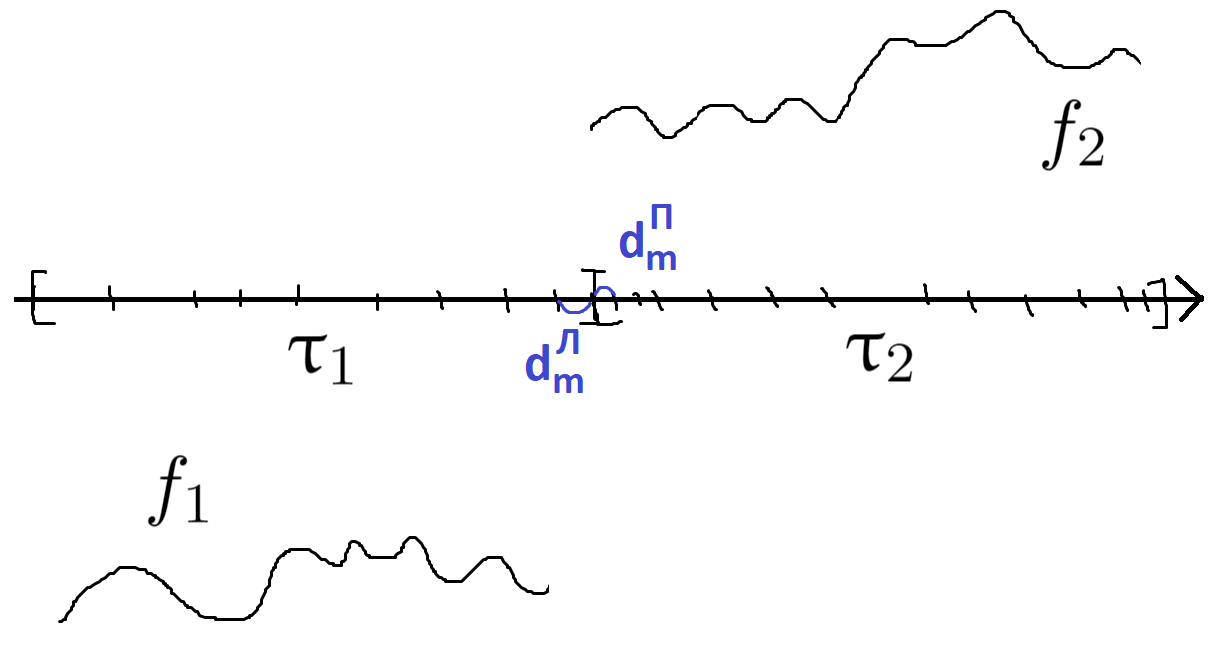
\includegraphics[width=5cm]{8_1}
		\end{figure}
		\[z \cdot \overline{z} = \abs{z}^2 \RA \frac{z_1}{z_2} := \frac{z_1 \cdot \overline{z_2}}{\abs{z_2}^2}\]
		\[k \in \R \RA \frac{z}{k} = \frac{x}{k} + i \frac{y}{k}\]
		Сложение действует как на векторах, что с умножением?\\
		Перейдем к полярной системе координат
		%рисунок 2 полярные координаты
		\begin{figure}[H]
	        \centering
	        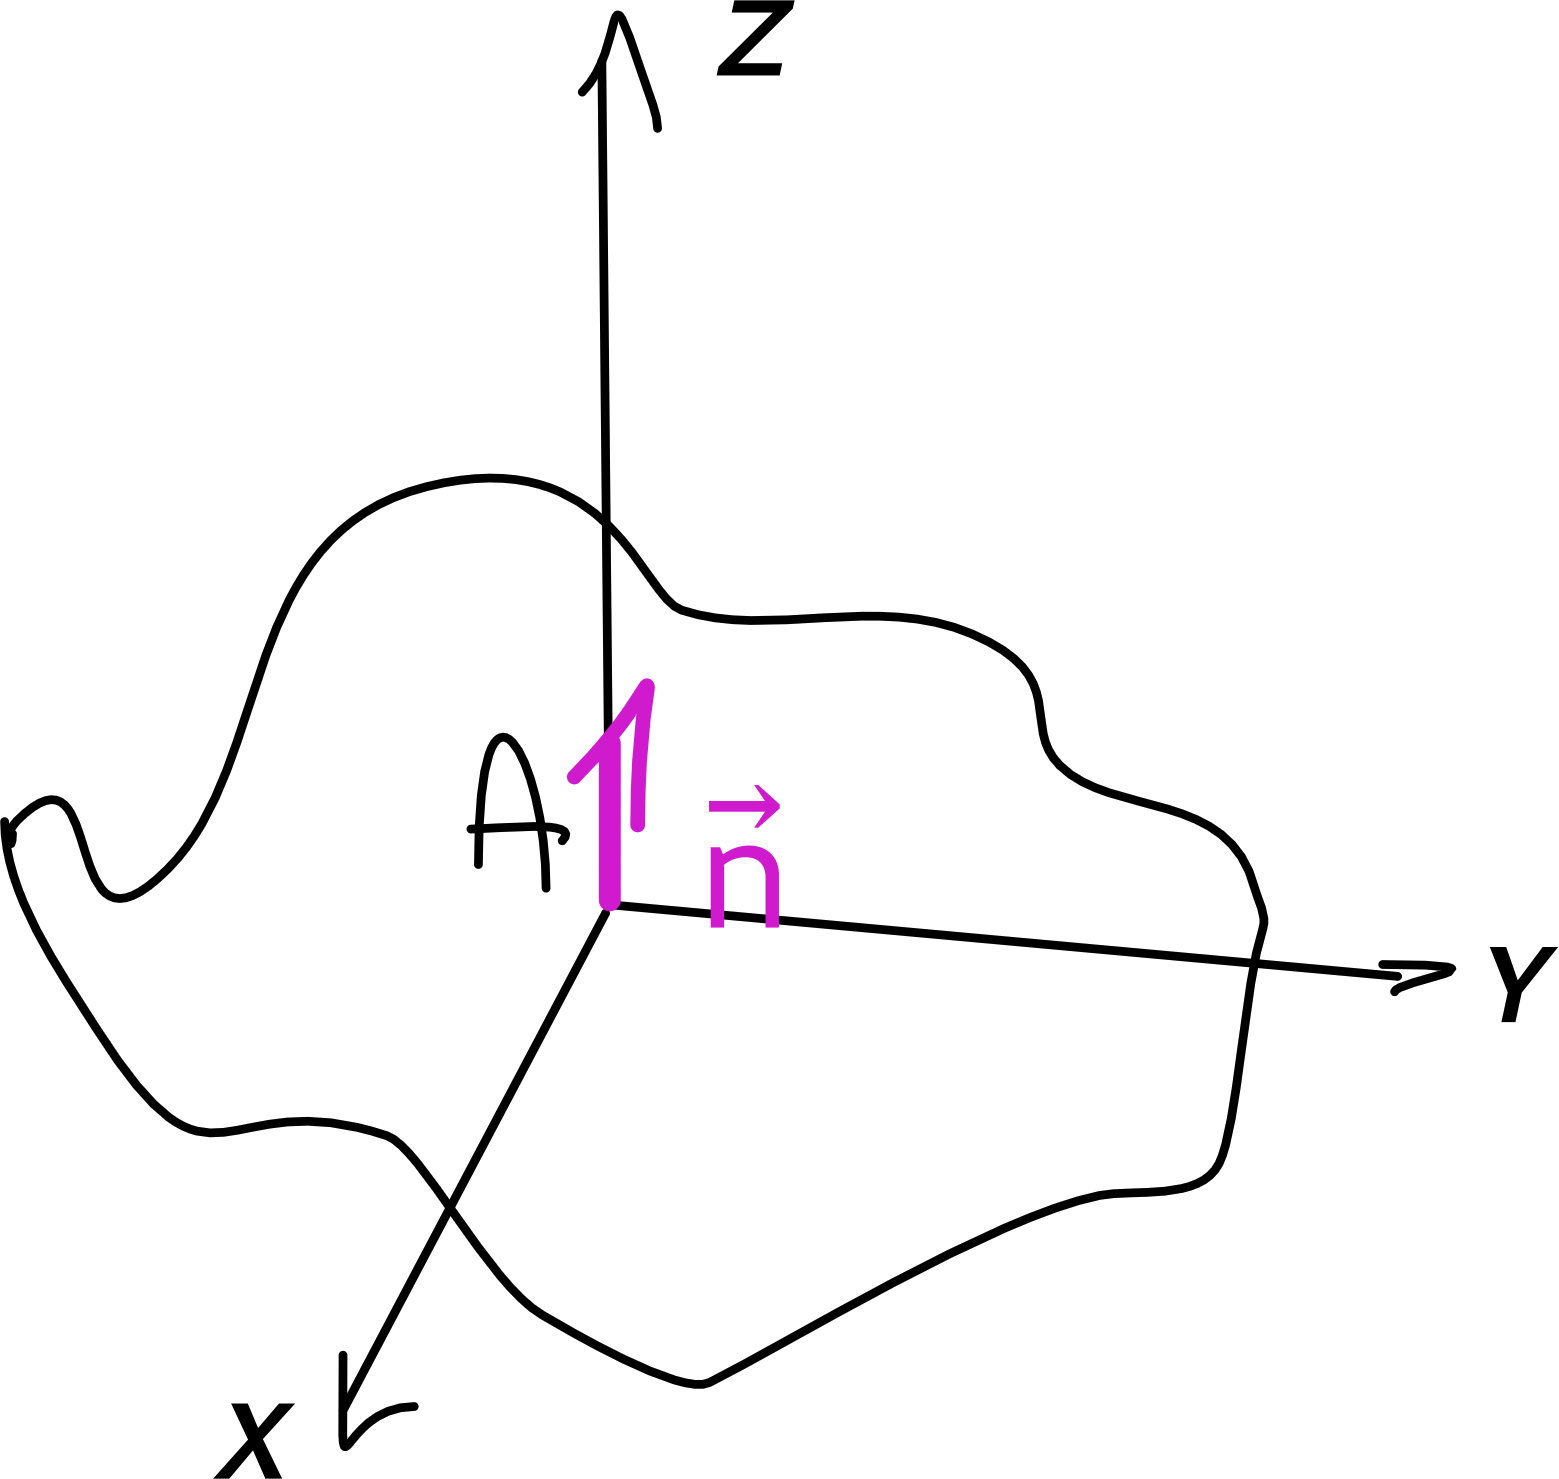
\includegraphics[width=5cm]{8_2}
		\end{figure}
		\[z = \abs{z} (\cos \varphi + i \sin \varphi)\]
		\[\real z = \abs{z} \cos \varphi\q \im z = \abs{z} \sin \varphi\]
		\[z_1 = \abs{z_1} (\cos \varphi_1 + i \sin \varphi_1)\q z_2 = \abs{z_2} (\cos \varphi_2 + i \sin \varphi_2)\]
		\begin{multline*}
			\Ra z_1 \cdot z_2 = \abs{z_1} \cdot \abs{z_2}
			(\cos \varphi_1 \cos \varphi_2 - \sin \varphi_1 \sin \varphi_2
		    +\\
			+i(\cos \varphi_1 \sin \varphi_2 + \sin \varphi_1 \cos \varphi_2)) =
		\end{multline*}
		\[ = \abs{z_1} \abs{z_2} (\cos(\varphi_1 + \varphi_2) +
		i \sin (\varphi_1 + \varphi_2))\]
		%рисунок 3
		\begin{figure}[H]
	        \centering
	        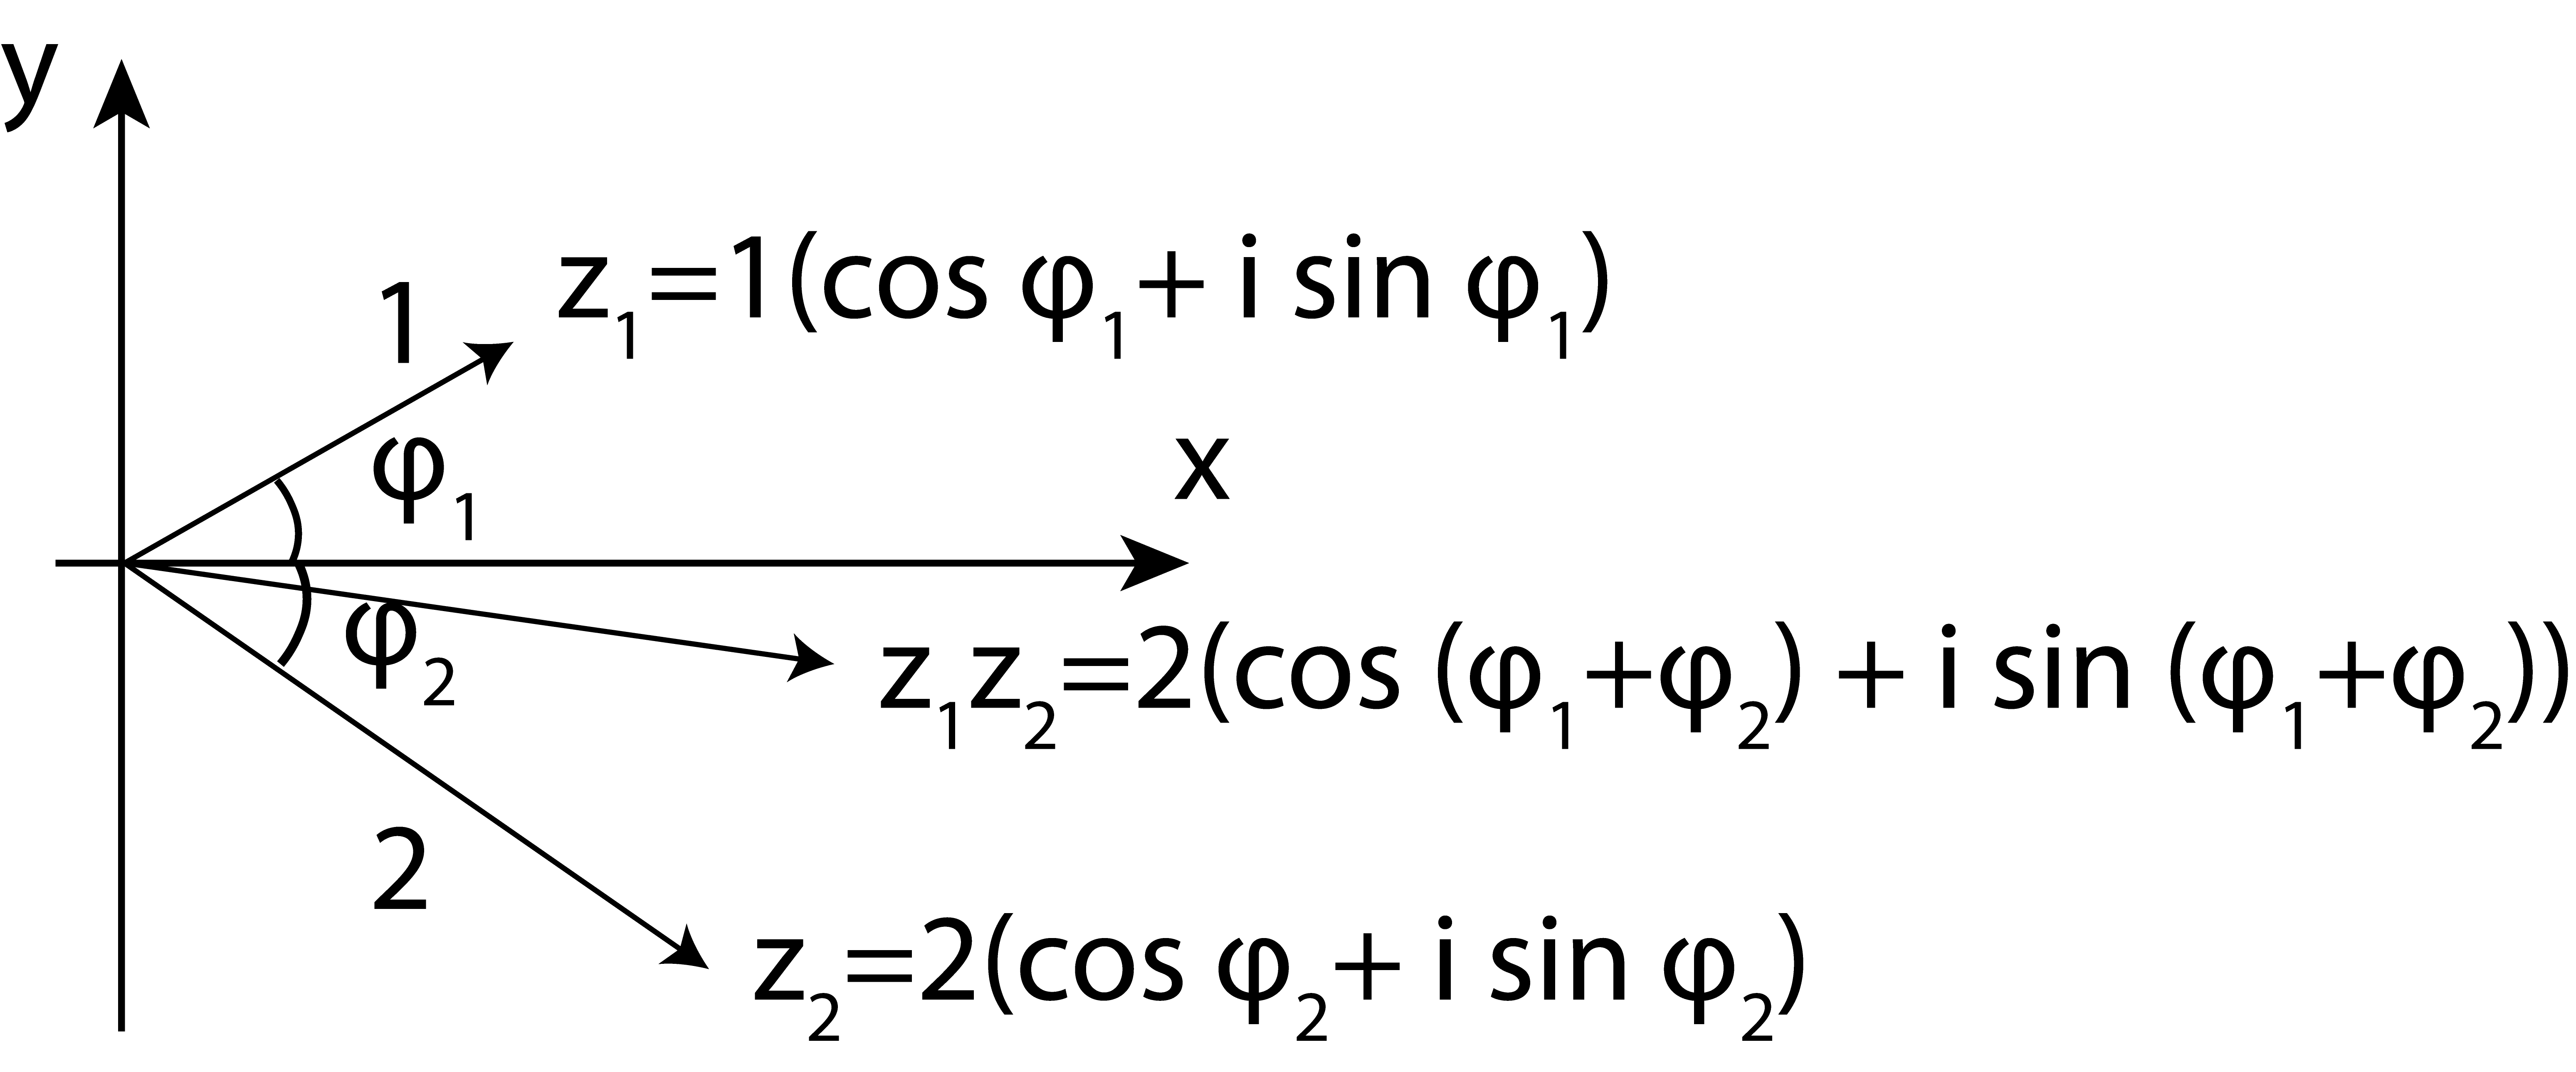
\includegraphics[width=7cm]{8_3}
		\end{figure}
	\end{Reminder}

	\begin{Theorem} [Ф-ла Муавра]
		\[z^n = \abs{z}^n (\cos{n \varphi} + i \sin n \varphi )\]
	\end{Theorem}

	\begin{Utv} [н-во $\bigtriangleup$]
		\[\abs{z_1 + z_2} \leq \abs{z_1} + \abs{z_2}\]
	\end{Utv}

	\begin{Theorem} [н-во Коши]
	    \[z_j, w_j \in \CC, \q j = 1, ..., n\]
		\[\abs{\sum_{j = 1}^n z_j \cdot w_j}^2 \leq \sum_{j = 1}^n
		\abs{z_j}^2 \cdot \sum_{j = 1}^n \abs{w_j}^2 \]
	\end{Theorem}

	\begin{Proof}
		\[\overline{ab} = \overline{a} \cdot \overline{b} \qq
		z + \overline{z} = 2 \real z \qq
		z - \overline{z} = 2 i \im z\]
		%\[0 \leq \sum_{j = 1}^n  \abs{z_j - \lambda w_j}^2 =
		%\sum_{j = 1}^n  (z_j - \lambda w_j) (\overline{z}_j -
		%\overline{\lambda} \overline{w}_j) = \sum( \abs{z}^2 + \abs{\lambda}^2
	    %\abs{w_j}^2 - \]
		%\[- (z_j \overline{\lambda} w_j + \overline{z}_j \lambda w_j) ) =
		%\sum \abs{z_j}^2 + \sum \abs{\lambda}^2 \abs{w_j}^2 - \sum 2 \real
		%\underbrace{(\overline{\lambda} \cdot z_j \cdot w_j)}\]
		\[0 \leq \sum_{j = 1}^n  \abs{z_j - \lambda \overline{w}_j}^2 =
		\sum \abs{z_j}^2 + \abs{\lambda}^2 \sum \abs{w_j}^2 - 2 \real
	    \Br{\sum_{j = 1}^n z_j \overline{\lambda} w_j}\]
		\[\lambda = \frac{\sum z_j w_j}{\sum \abs{w_j}^2}\]
		\[0 \leq \sum \abs{z_j}^2 + \frac{\abs{\sum z_j w_j}^2}
		{(\sum \abs{w_j}^2)^2} \cdot \sum \abs{w_j}^2 -
	    2 \real \left[  \frac{\sum \overline{z_j} \cdot \overline{w_j}}
        {\sum \abs{w_j}^2} \sum_{j = 1}^n z_j w_j \right]\]
		\[\text{hint: } [...] \leq \frac{\abs{\sum z_j w_j}^2}{\sum \abs{w_j}^2}\]
		\[0 \leq \sum \abs{z_j}^2 + \frac{\abs{\sum z_j w_j}^2}{\sum \abs{w_j}} -
		2 \frac{\abs{\sum z_j w_j}^2}{\sum \abs{w_j}^2}\]
		\[\abs{\sum^n_{j = 1} z_j w_j}^2 \leq \sum^n_{j = 1} \abs{z_j}^2 \cdot
		\sum_{j = 1}^n \abs{w_j}^2 \]
	\end{Proof}

	\begin{definition}
	    \ul{Комплексная последовательность} $c_n \in \CC$
		\[c_n = a_n + i b_n,\q a_n, b_n \in \R\]
		\[c_n \to c \in \CC \rla \abs{c_n - c} \to 0 \rla \begin{cases}
				a_n \to a\\
				b_n \to b
		\end{cases}\]
		\[\rla \text{При } n \to \infty \qq \text{ т.е } \ \begin{align}
				\real c_n \to \real c\\
				\im c_n \to \im c
		\end{align}\]
		\[\rla \{c_n\}_{n \in \N} \text{ - сх. в себе}\]
	\end{definition}

	\newpage
	\subsection{Дробно-линейное  отображение.  Круговое  свойство.  Другие  св-ва (б/д)}

	\begin{examples} [функций к. п.]
		\begin{enumerate}
			\item $ \us{\text{зафикс.}}{a \in \CC}  \qq f(z) = z + a \qq f: \CC \to \CC$\\
				парал. перенос вдоль вектора $\overline{a} = (\real a, \im a)$
				%рисунок 4
				\begin{figure}[H]
		            \centering
		            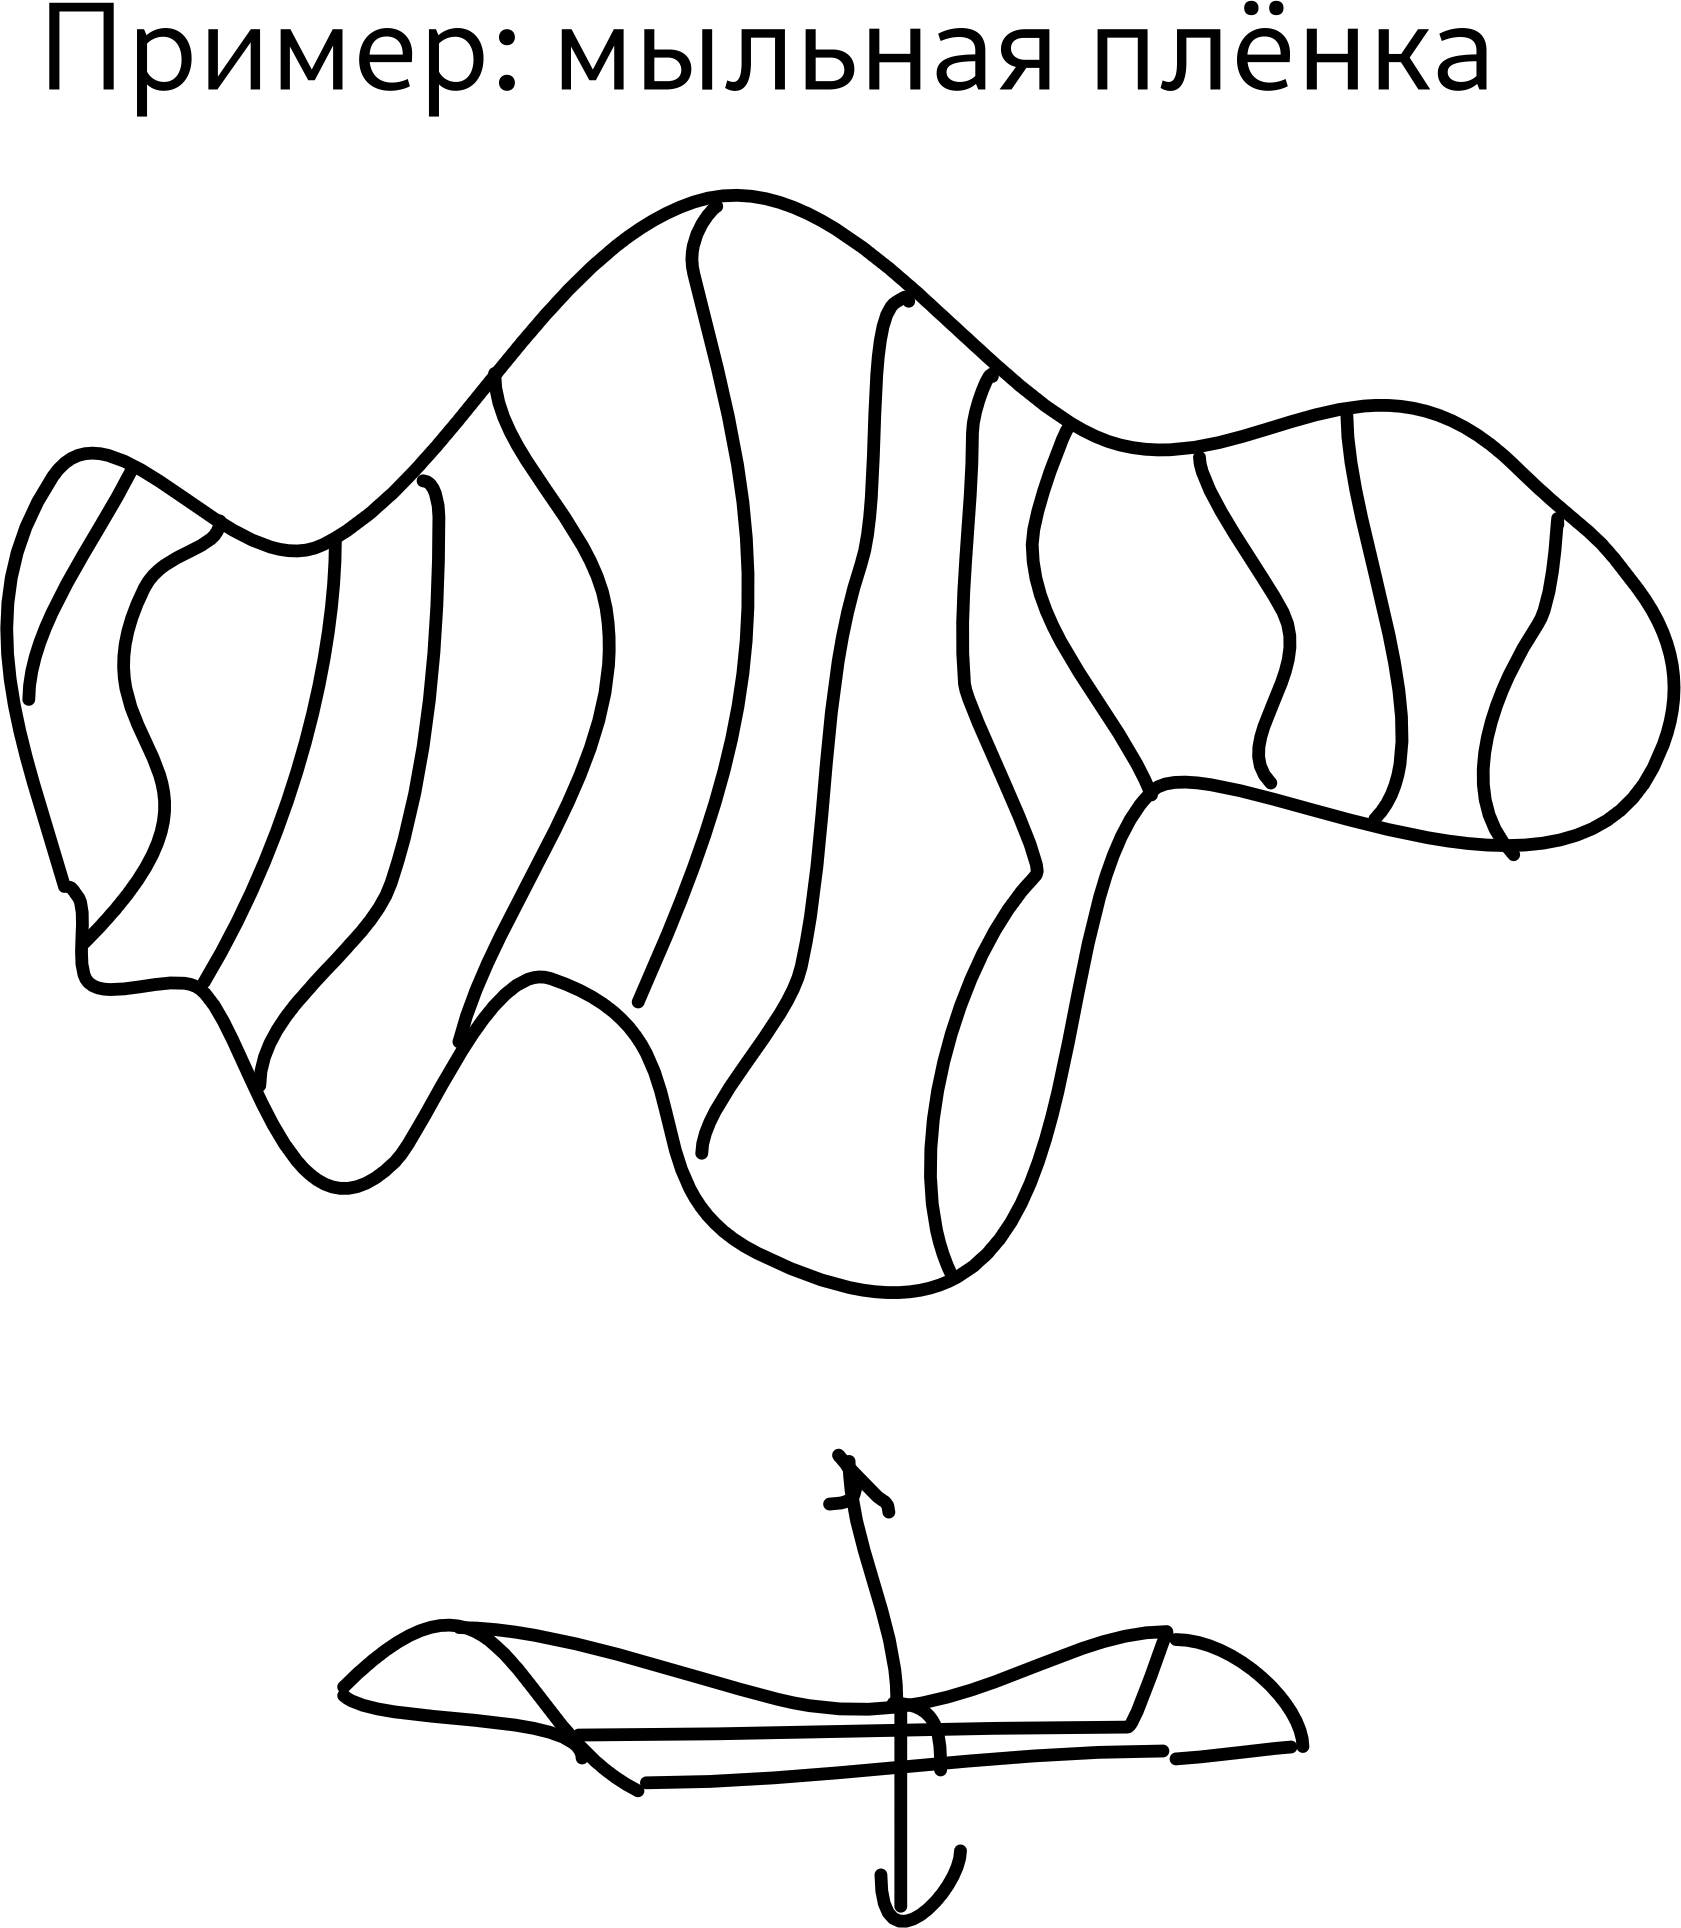
\includegraphics[width=5cm]{8_5}
				\end{figure}
			\item $\lambda \in \CC \q \abs{\lambda} = 1 \q \lambda = \cos \Theta + i \sin \Theta \q
				z = \abs{z}(\cos \varphi + i \sin \varphi)$
				\[f(z) = \lambda z = \abs{z} (\cos(\varphi + \Theta) + i \sin (\varphi + \Theta))\]
				Поворот вокруг O на угол $\Theta$ против часовой стрелки
				%рисунок 5
				\begin{figure}[H]
		            \centering
		            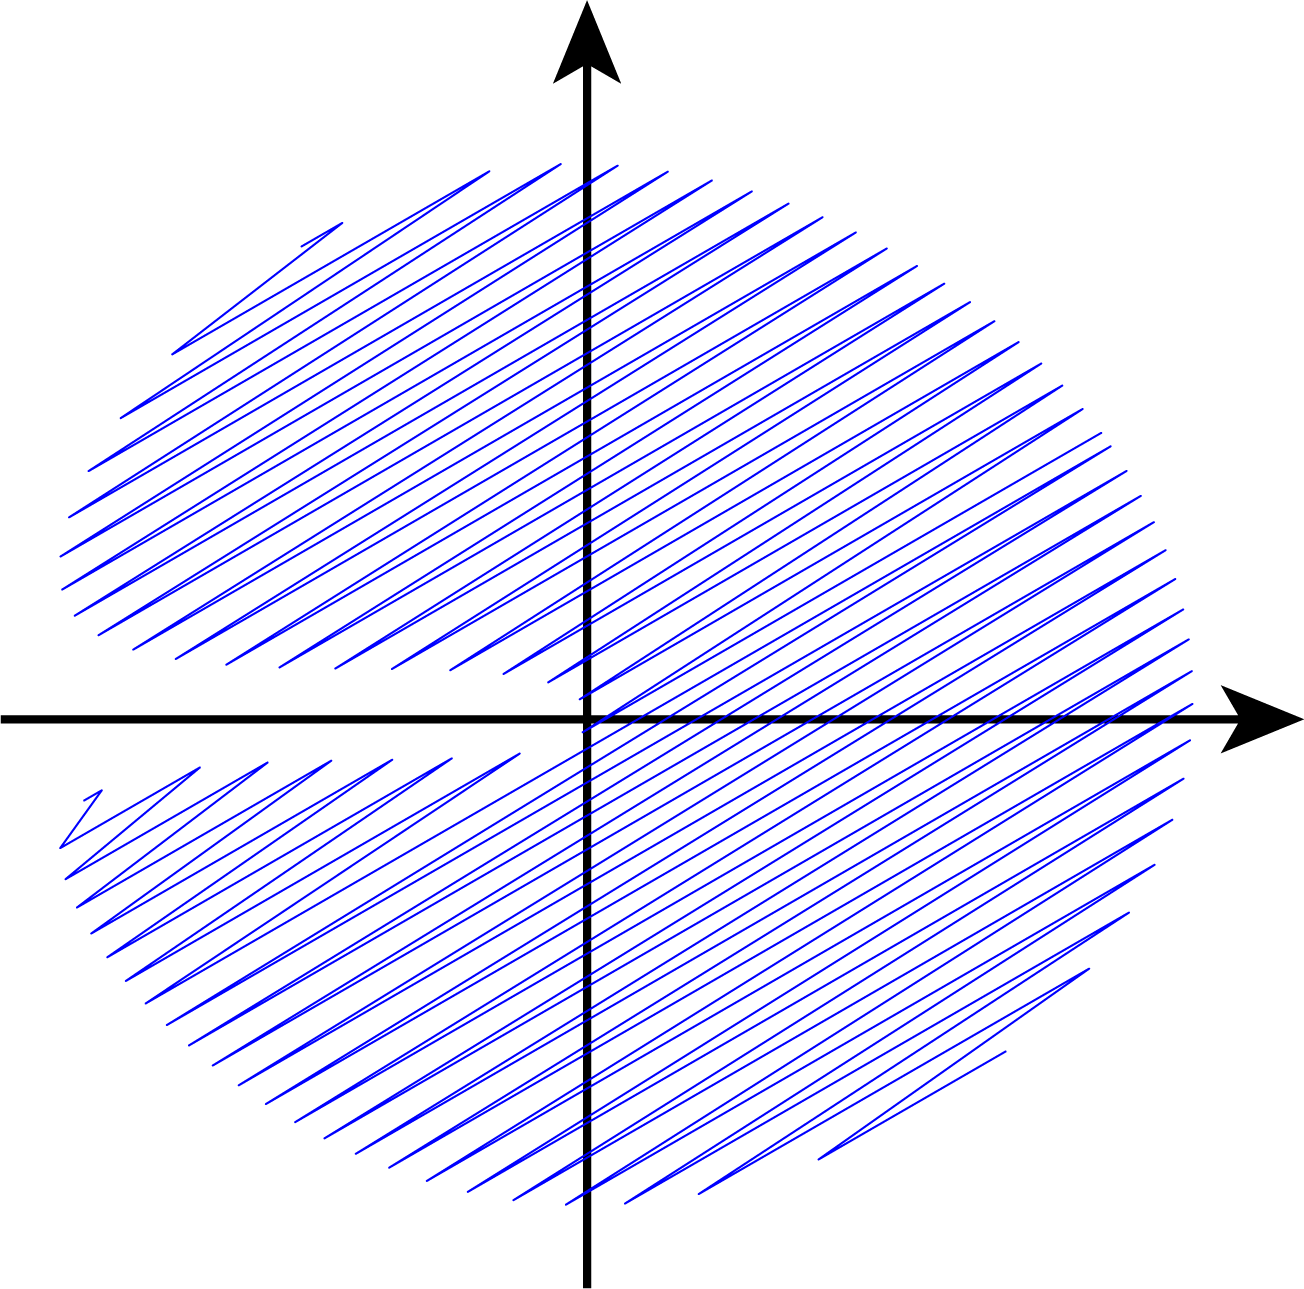
\includegraphics[width=5cm]{8_6}
				\end{figure}
			\item $k \in [0, +\infty)$
				\[f(z) = k z = k \cdot \abs{z} (\cos \varphi + i \sin \varphi)\]
				\[\abs{f(z)} = k \abs{z}\]
				Гомотетия с коэф. $k$
			\item $f(z) = z^2 = \abs{z}^2 (\cos 2\varphi + i \sin 2\varphi)$
				%рисунок 6
				\begin{figure}[!h]
		            \centering
		            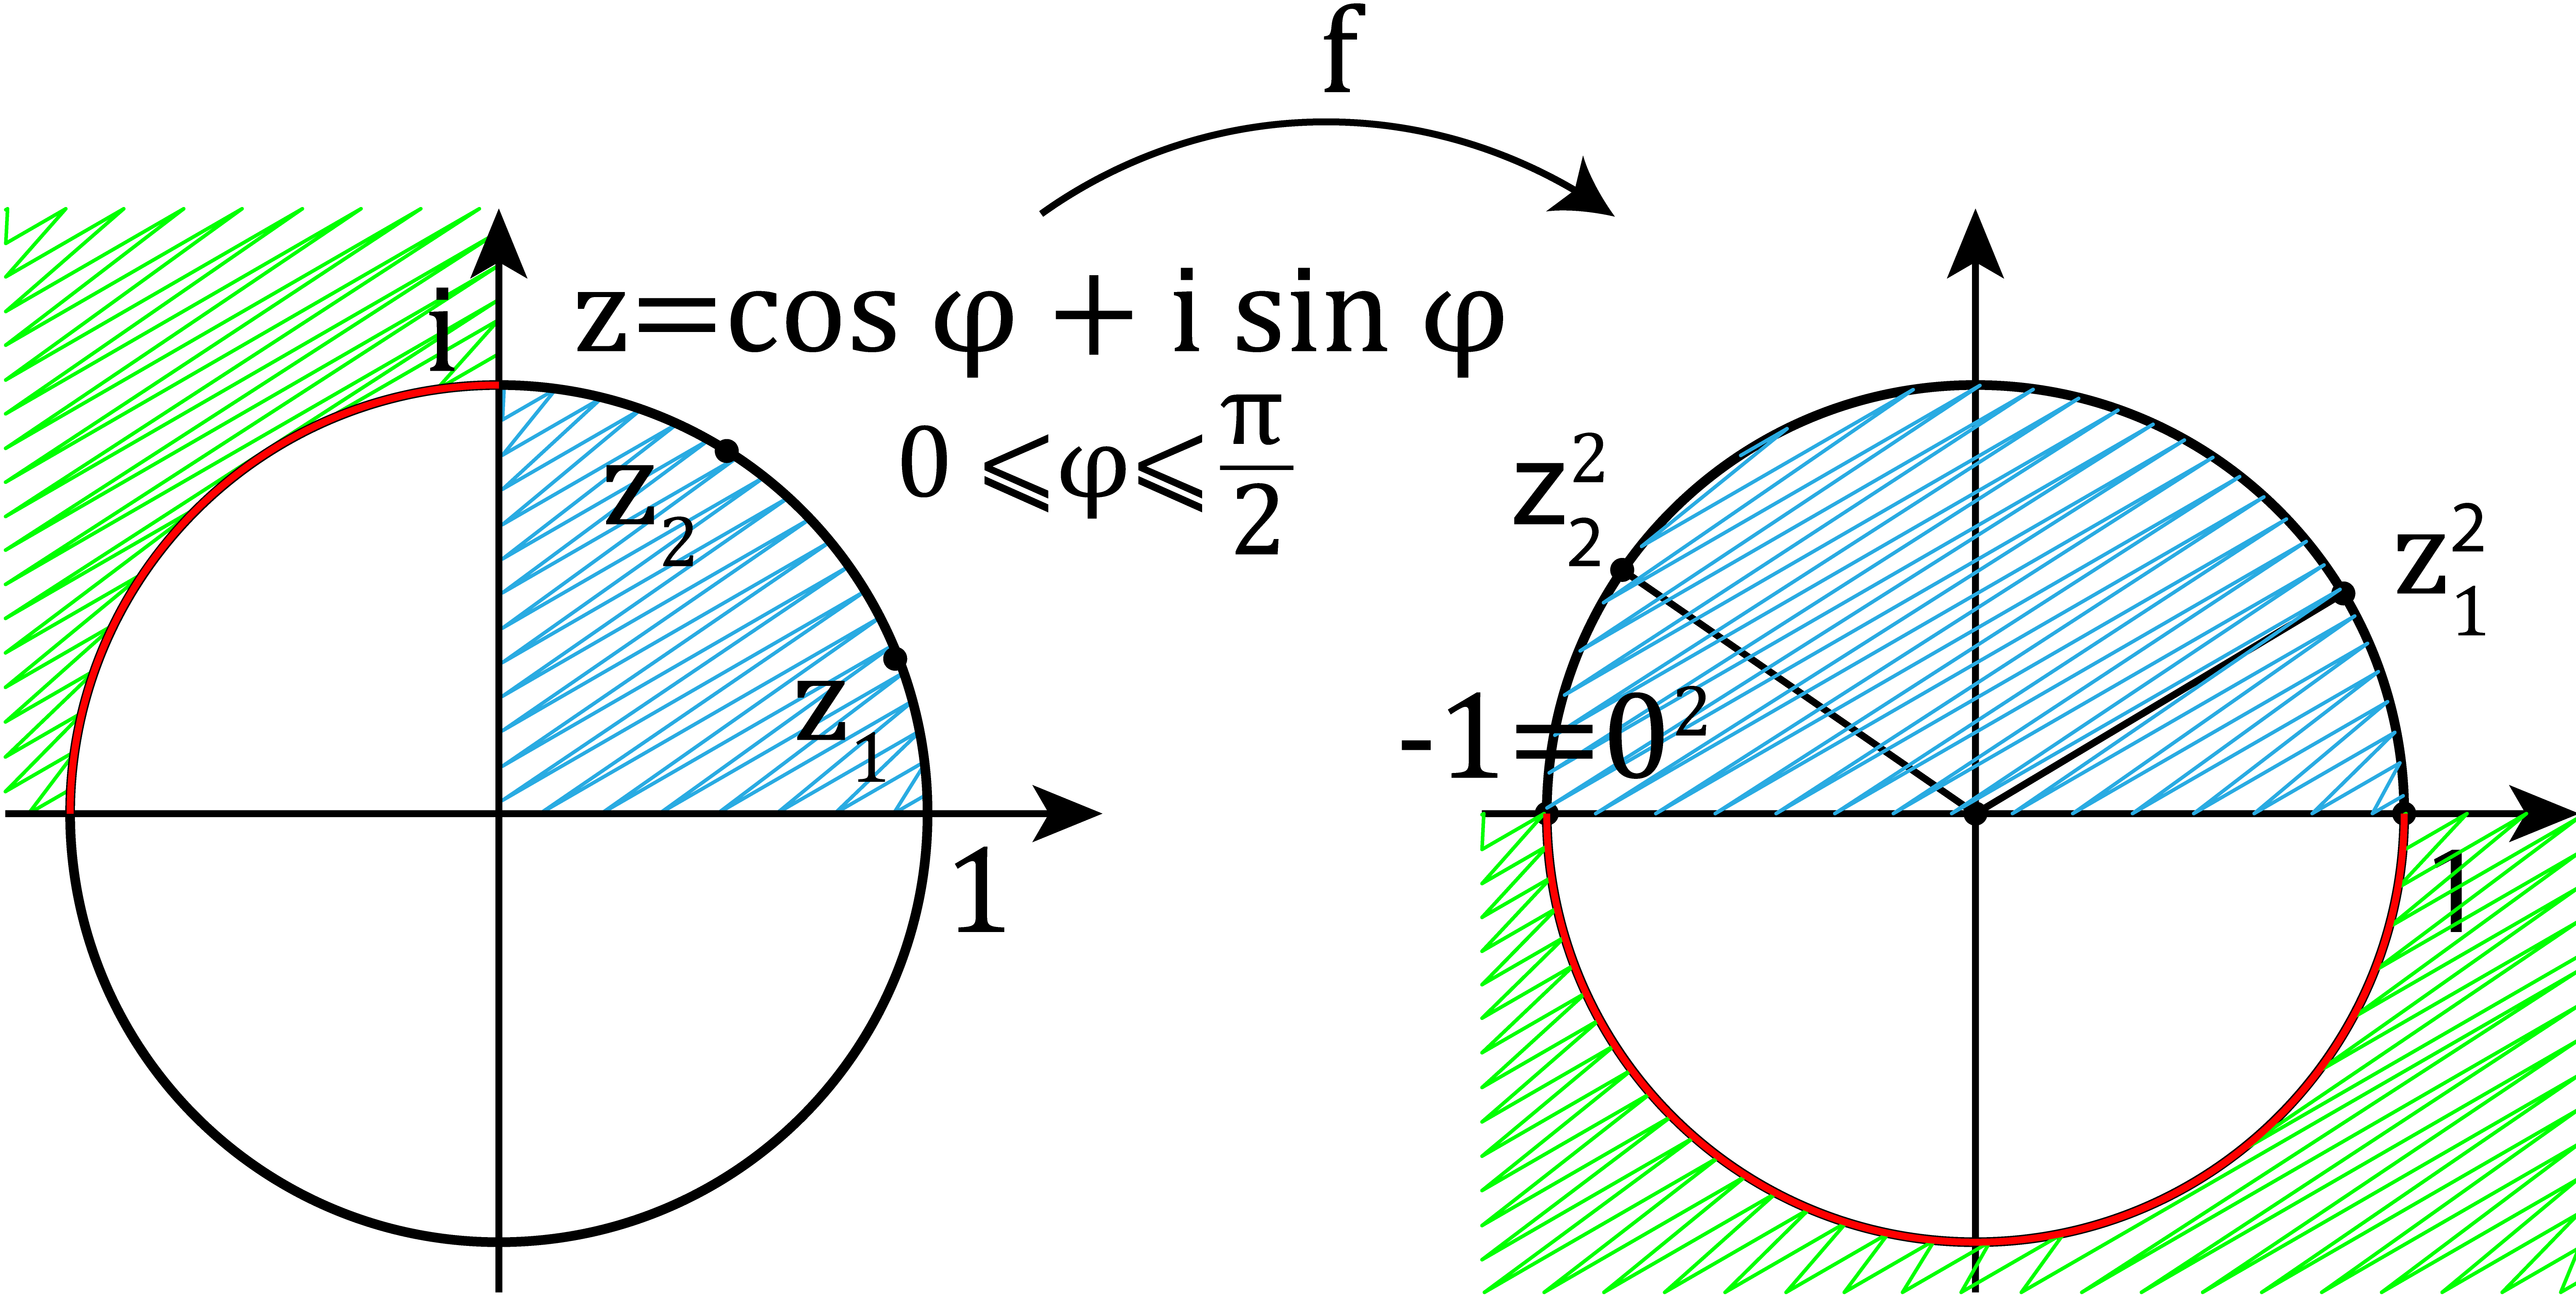
\includegraphics[width=8cm]{8_7}
				\end{figure}
				\[z :\ \abs{z} < 1 \qq\q \Ra z :\ \abs{z} < 1\]
				\[0 \leq \varphi \leq \frac{\pi}{2} \qq\q 0 \leq \varphi \leq \pi\]
			\item Инверсия (относительно ед. окружности)
				\[f(z) = \frac{1}{z} \qq f: \CC \setminus \{0\} \to \CC\]
				\[f(z) = \frac{\overline{z}}{\abs{z}^2}\]
				%рисунок 7
				\begin{figure}[!h]
		            \centering
		            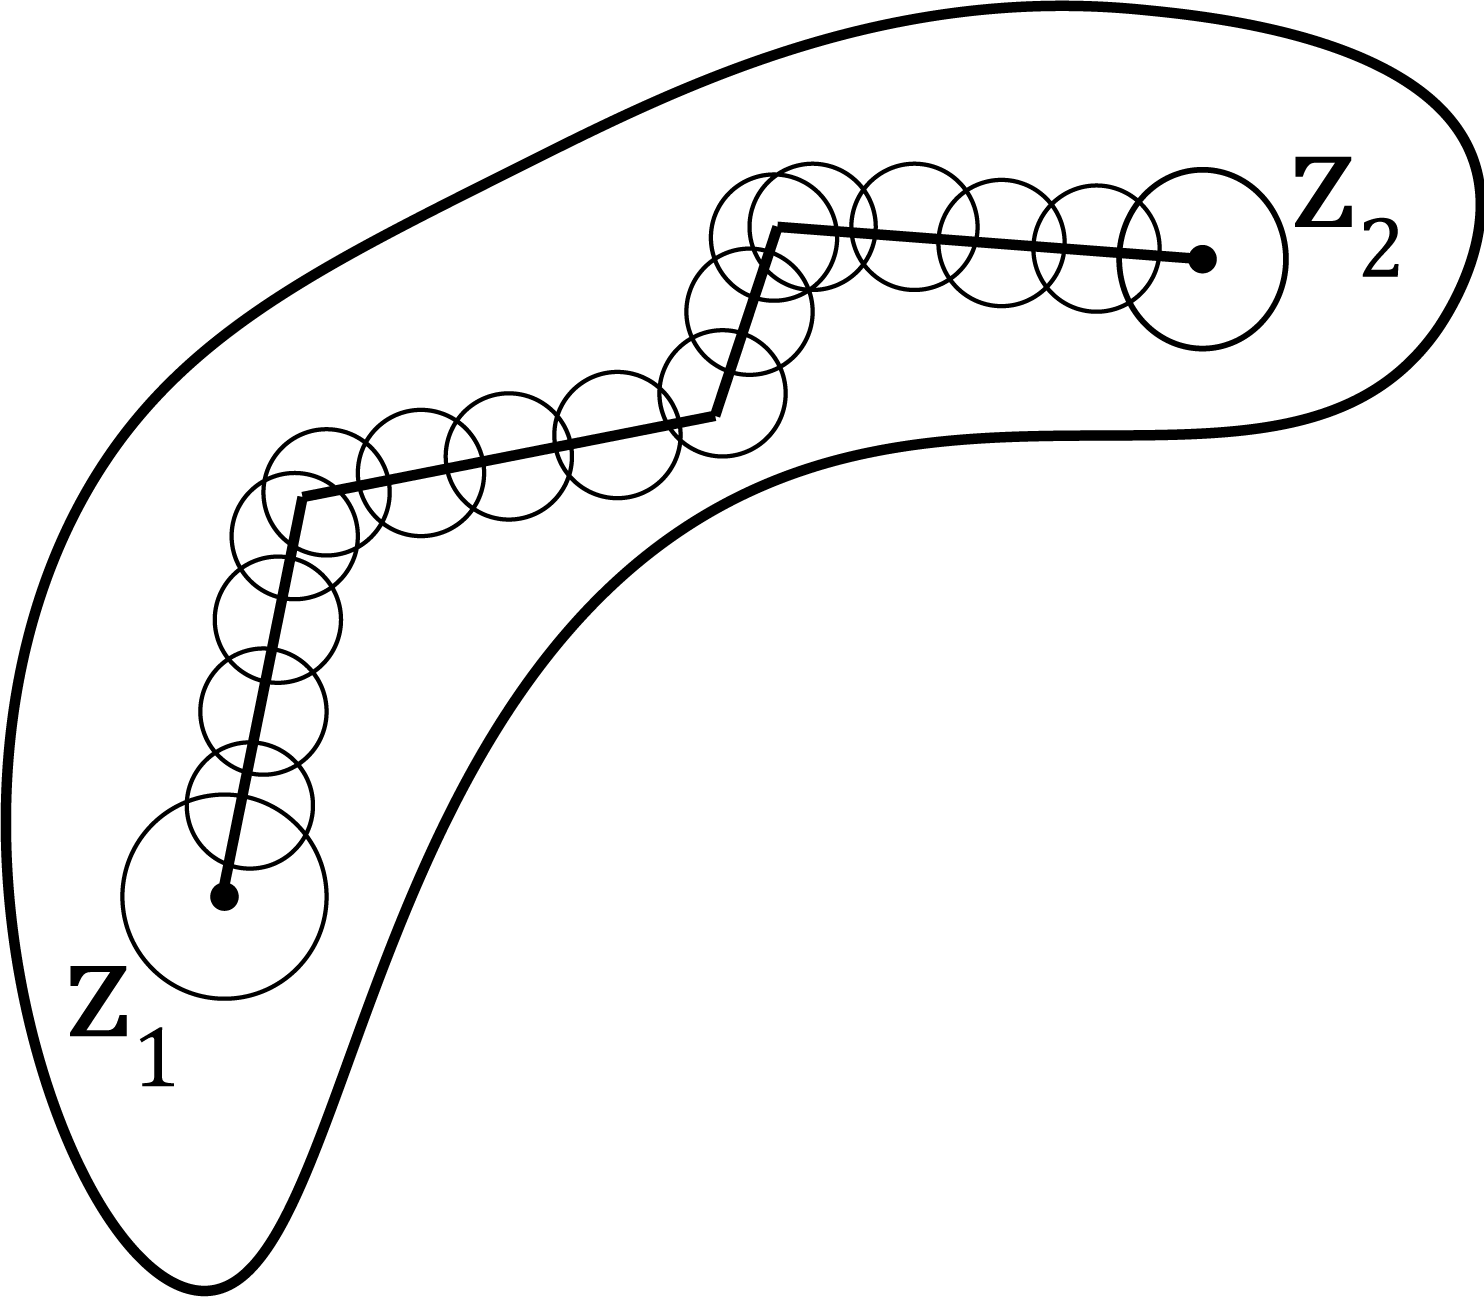
\includegraphics[width=8cm]{8_8}
				\end{figure}
				Какие точки останутся неподвижными? Их ровно две $-1$ и $1$
				$\left(\displaystyle z = \frac{1}{z}\right)$
			\item Дробно-линейные отобр-я (преобр. Мёбиуса)
				\[L(z) = \frac{az + b}{cz + d} \qq (c, d) \neq (0, 0)\]
				\[\text{Если } c = 0, \text{ то } L \text{ - афинное преобразование, т.е композиция }\]
				гомотетий, поворотов и пар. переносов
				\[L : \CC \setminus \{- \frac{d}{c}\} \to \CC\]
				\[\text{Если } \begin{vmatrix}
					a & b\\
					c & d
				\end{vmatrix} = 0, \text{ то } L(z) = const\]
				Доопр. инв. $\displaystyle f(z) = \frac{1}{z} \qq f(0) = \infty \qq f(\infty) = 0$
				\[L \text{ --- доопределим}\]
				\[L(- \frac{d}{c}) = \infty  \qq L(\infty) = \frac{a}{c}\]
				\[\text{Тогда } L : \hat{\CC} \to \hat{\CC} \text{ - вз. однозн., если }
				\begin{vmatrix}
					a & b\\
					c & d
				\end{vmatrix} \neq 0\]
				\[w = \frac{az + b}{cz + d}\]
				\[czw + dw = az + b\]
				\[z(cw - a) = b - dw\]
				\[z = \frac{b - dw}{cw - a} \qq \begin{vmatrix}
					-d & b\\
					c & -a
				\end{vmatrix} = ad - bc \neq 0 \]

		\end{enumerate}\\
		\text{ }\\
		\\Сфера римана $\rla \overline{\CC} = \CC \cup \{\infty\}$
		\begin{figure}[H]
			\centering
			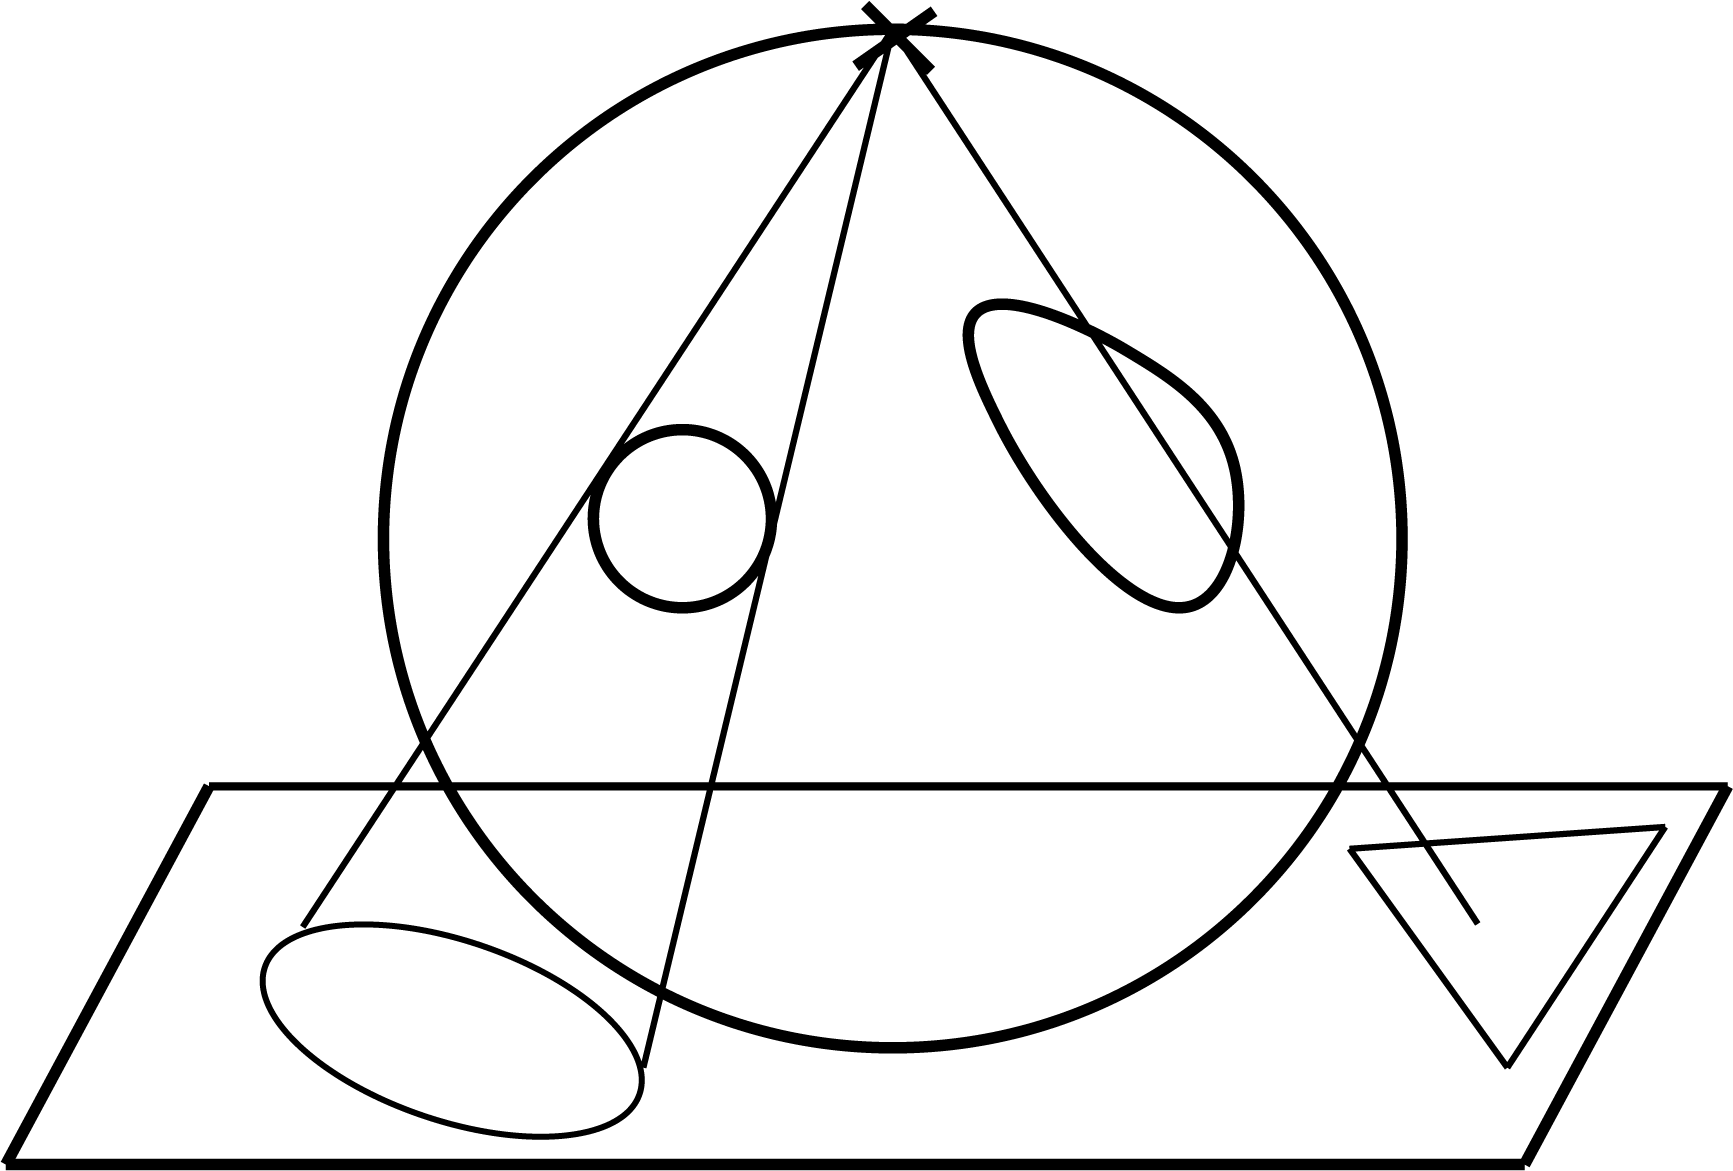
\includegraphics[width=5cm]{8_9}
		\end{figure}
	\end{examples}
	\begin{utv}
		Если известно, что $L(z_1) = w_1 \qq L(z_2) = w_2 \qq L(z_3) = w_3$
		\[\Ra \text{ можно восстановить дробно-лин. отобр } L\]
		\[z_1 \neq z_2 \neq z_3 \qq w_1 \neq w_2 \neq w_3\]
	\end{utv}

	\begin{definition}
	    Обобщенная окр-ть $=$ окр-ть или прямая
	\end{definition}

	\begin{utv} [круговое св-во]
		Дробно-лин отобр. переводит обобщенные окр. в обобщ. окр.
	\end{utv}

	\begin{proof}
		Дробно-лин. отобр - композиция
		\begin{enumerate}
			\item Гомотетий
			\item Пар. переносов
			\item Поворотов
			\item Инверсий
		\end{enumerate}
		\[1 - 3 \text{ - переводят окр. } \to \text{ окр.}, \q \text{прямые } \to \text{ прямые}\]
		Надо разобраться, что делает инверсия с окр.
		\[\alpha \cdot \abs{z}^2 + \beta \real z + \gamma \im z + \delta = 0\]
		\[\alpha, \beta, \gamma, \delta \in \R\]
		\[\alpha(x^2 + y^2) + \beta x + \gamma y + \delta = 0\]
		\[\alpha = 0 \text{ --- прямые}\]
		\[\alpha \neq 0 \text{ --- окружности}\]
		\[x^2 + y^2 + \frac{\beta}{\alpha} x + \frac{\gamma}{\alpha}y + \frac{\delta}{\alpha} = 0\]
		\[\left(x + \frac{\beta}{2\alpha}\right)^2 + \left(y + \frac{\gamma}{2 \alpha}\right)^2
		+ \frac{\delta}{\alpha} - \frac{\beta ^2 + \gamma^2 }{4 \alpha^2} = 0\]
		\[4\alpha \delta \leq \beta^2 + \gamma^2\]
		\[z \ra \frac{1}{z} = \frac{\overline{z}}{\abs{z}^2} = \frac{x - iy}{\abs{z}^2}\]
		\[\alpha \cdot \frac{1}{\abs{z}^2} + \beta \frac{\real z}{\abs{z}^2} -
		\gamma \frac{\im z}{\abs{z}^2} + \delta = 0\]
		\[\alpha + \beta \real z - \gamma \im z + \delta \abs{z}^2 = 0\]
		\[4 \alpha \delta \leq \beta^2 + \gamma^2\]
	\end{proof}

	\begin{Definition} [симметрия отн. окружности]\
	    %рисунок8 кружок
		\begin{figure}[H]
	        \centering
	        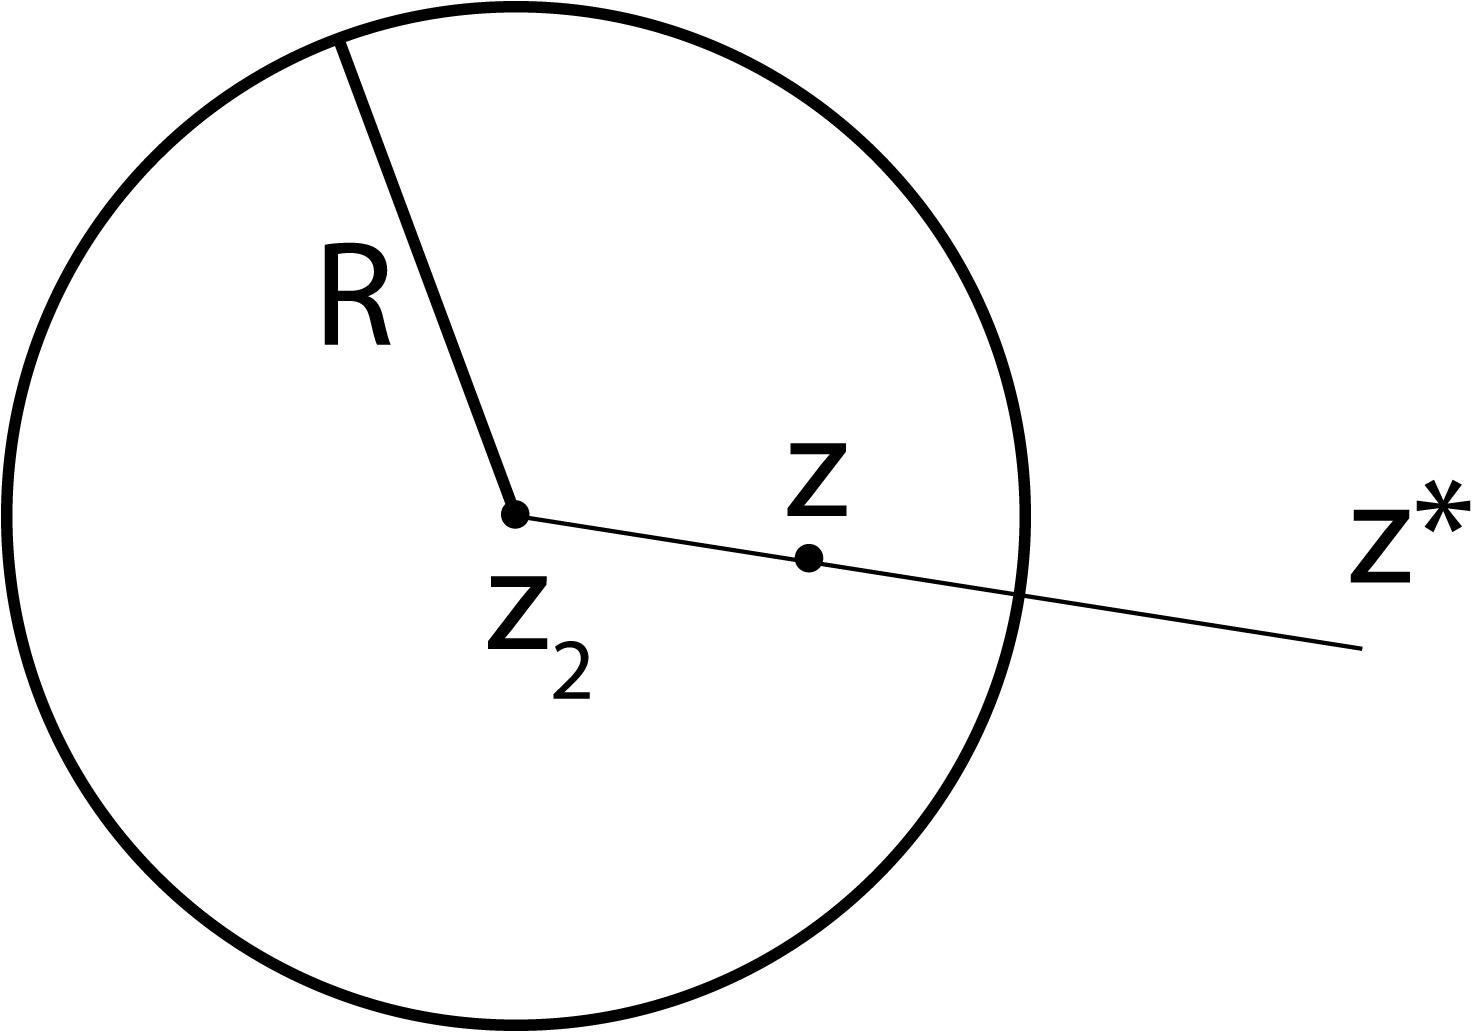
\includegraphics[width=5cm]{8_10}
      	\end{figure}
		\[\abs{z^* - z_0} \cdot \abs{z - z_0} = R^2\]
		\[z^* \text{ --- симметрична } z \text{ отн окр. } \abs{z - z_0} = R\]
		Рассмотрим
		%рисунок 9 отобр из кружка в плоскость
		\begin{figure}[H]
	        \centering
	        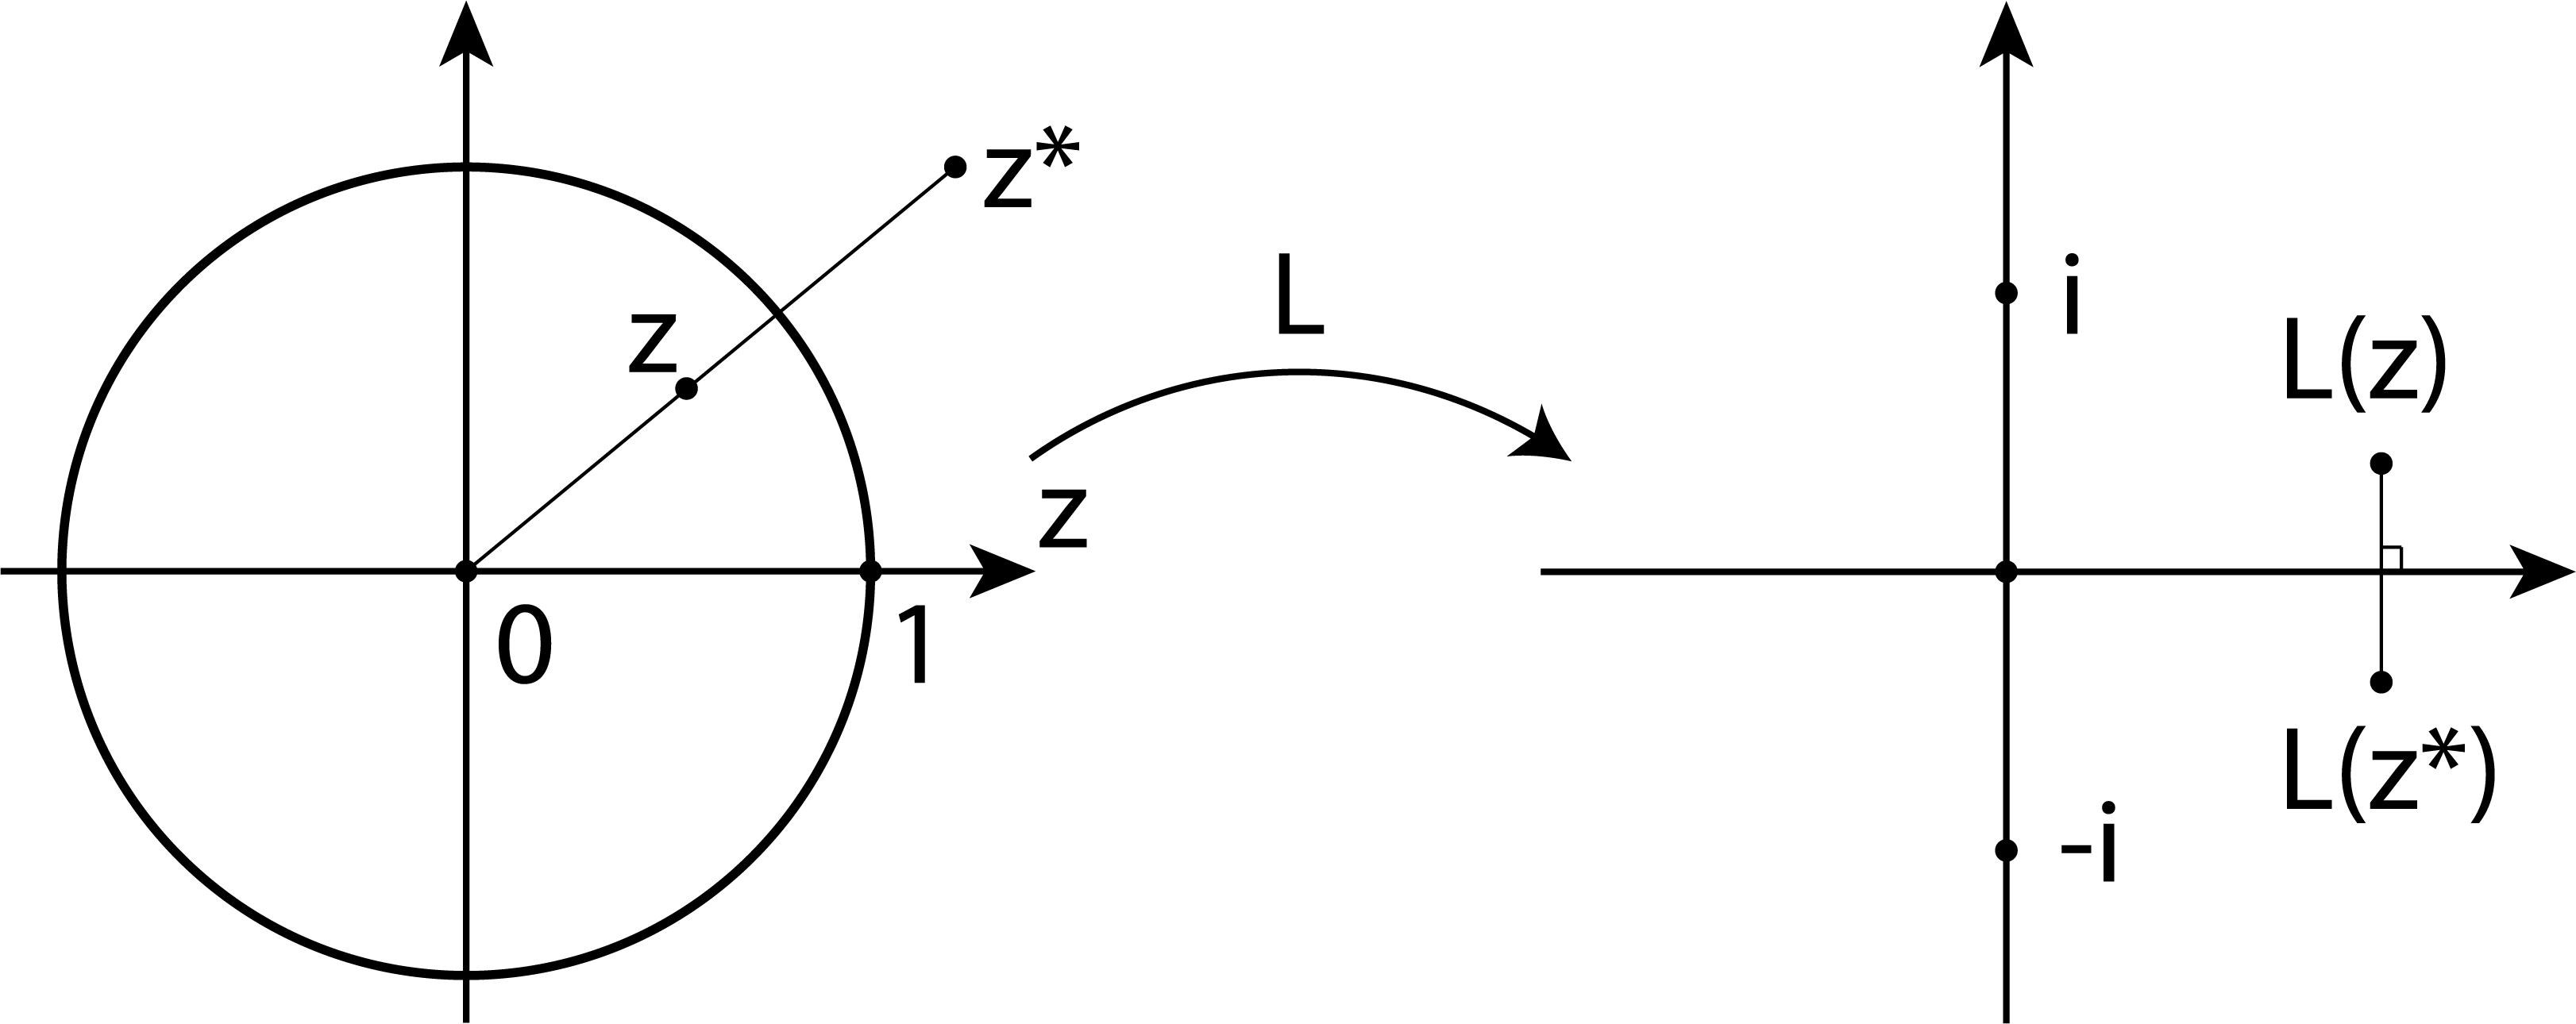
\includegraphics[width=8cm]{8_11}
		\end{figure}
		\[z^* = \frac{1}{\abs{z}}(\cos \varphi + i \sin \varphi) =
		\frac{1}{\abs{z}} \cdot \frac{z}{\abs{z}}\]
		\[\begin{align}
			&L: & L(y) = \frac{z + b}{cz + d}\\
			&L(0) = i & L(0) = i = \frac{b}{d}\\
			&L(-1) = 0 & L(-1) = \frac{b - 1}{d - c} = 0\\
			&L(1) = \infty & L(1) = \frac{1 + b}{c + d} = \infty\\
		\end{align}\]
		\[b = 1 \qq d = -i \qq \frac{1 + 1}{c - i} = \infty \q c = i\]
		\[L(z) = \frac{z + 1}{iz - i} = -i \frac{z + 1}{z - 1}\]
		\[L(z) = -i \frac{z + 1}{z - 1} \]
		\[L(z^*) = -i \frac{\frac{z}{\abs{z}^2} + 1}{\frac{z}{\abs{z}^2} - 1} =
		-i \frac{z + \abs{z}^2}{z - \abs{z}^2}\]
		\[\overline{L(z)} = \overline{-i} \frac{(\overline{z} + 1) ^2 z}{(\overline{z} - 1)^2 z} =
		i \frac{\abs{z}^2 + z}{\abs{z}^2 - z} = L(z^*)\]

	\end{Definition}

	\begin{Example}
		\[7) \q f(z) = e^z = e^{x + iy} = e^x (\cos y + i\sin y) \text{ (по ф. Эйлера)}\]
		\[e^{iy} = \cos y + i \sin y \]
		\[e^{i\pi} = -1 \q  \text{ Замечательная формула, которая связывает 3 числа}\]
		\[(x, y) \os{e^z}{\to } (e^x \cos y;\ e^x \sin y)\]
		%рисунок10 преобразование $e^z$ с солнышком
		\begin{figure}[H]
			\centering
			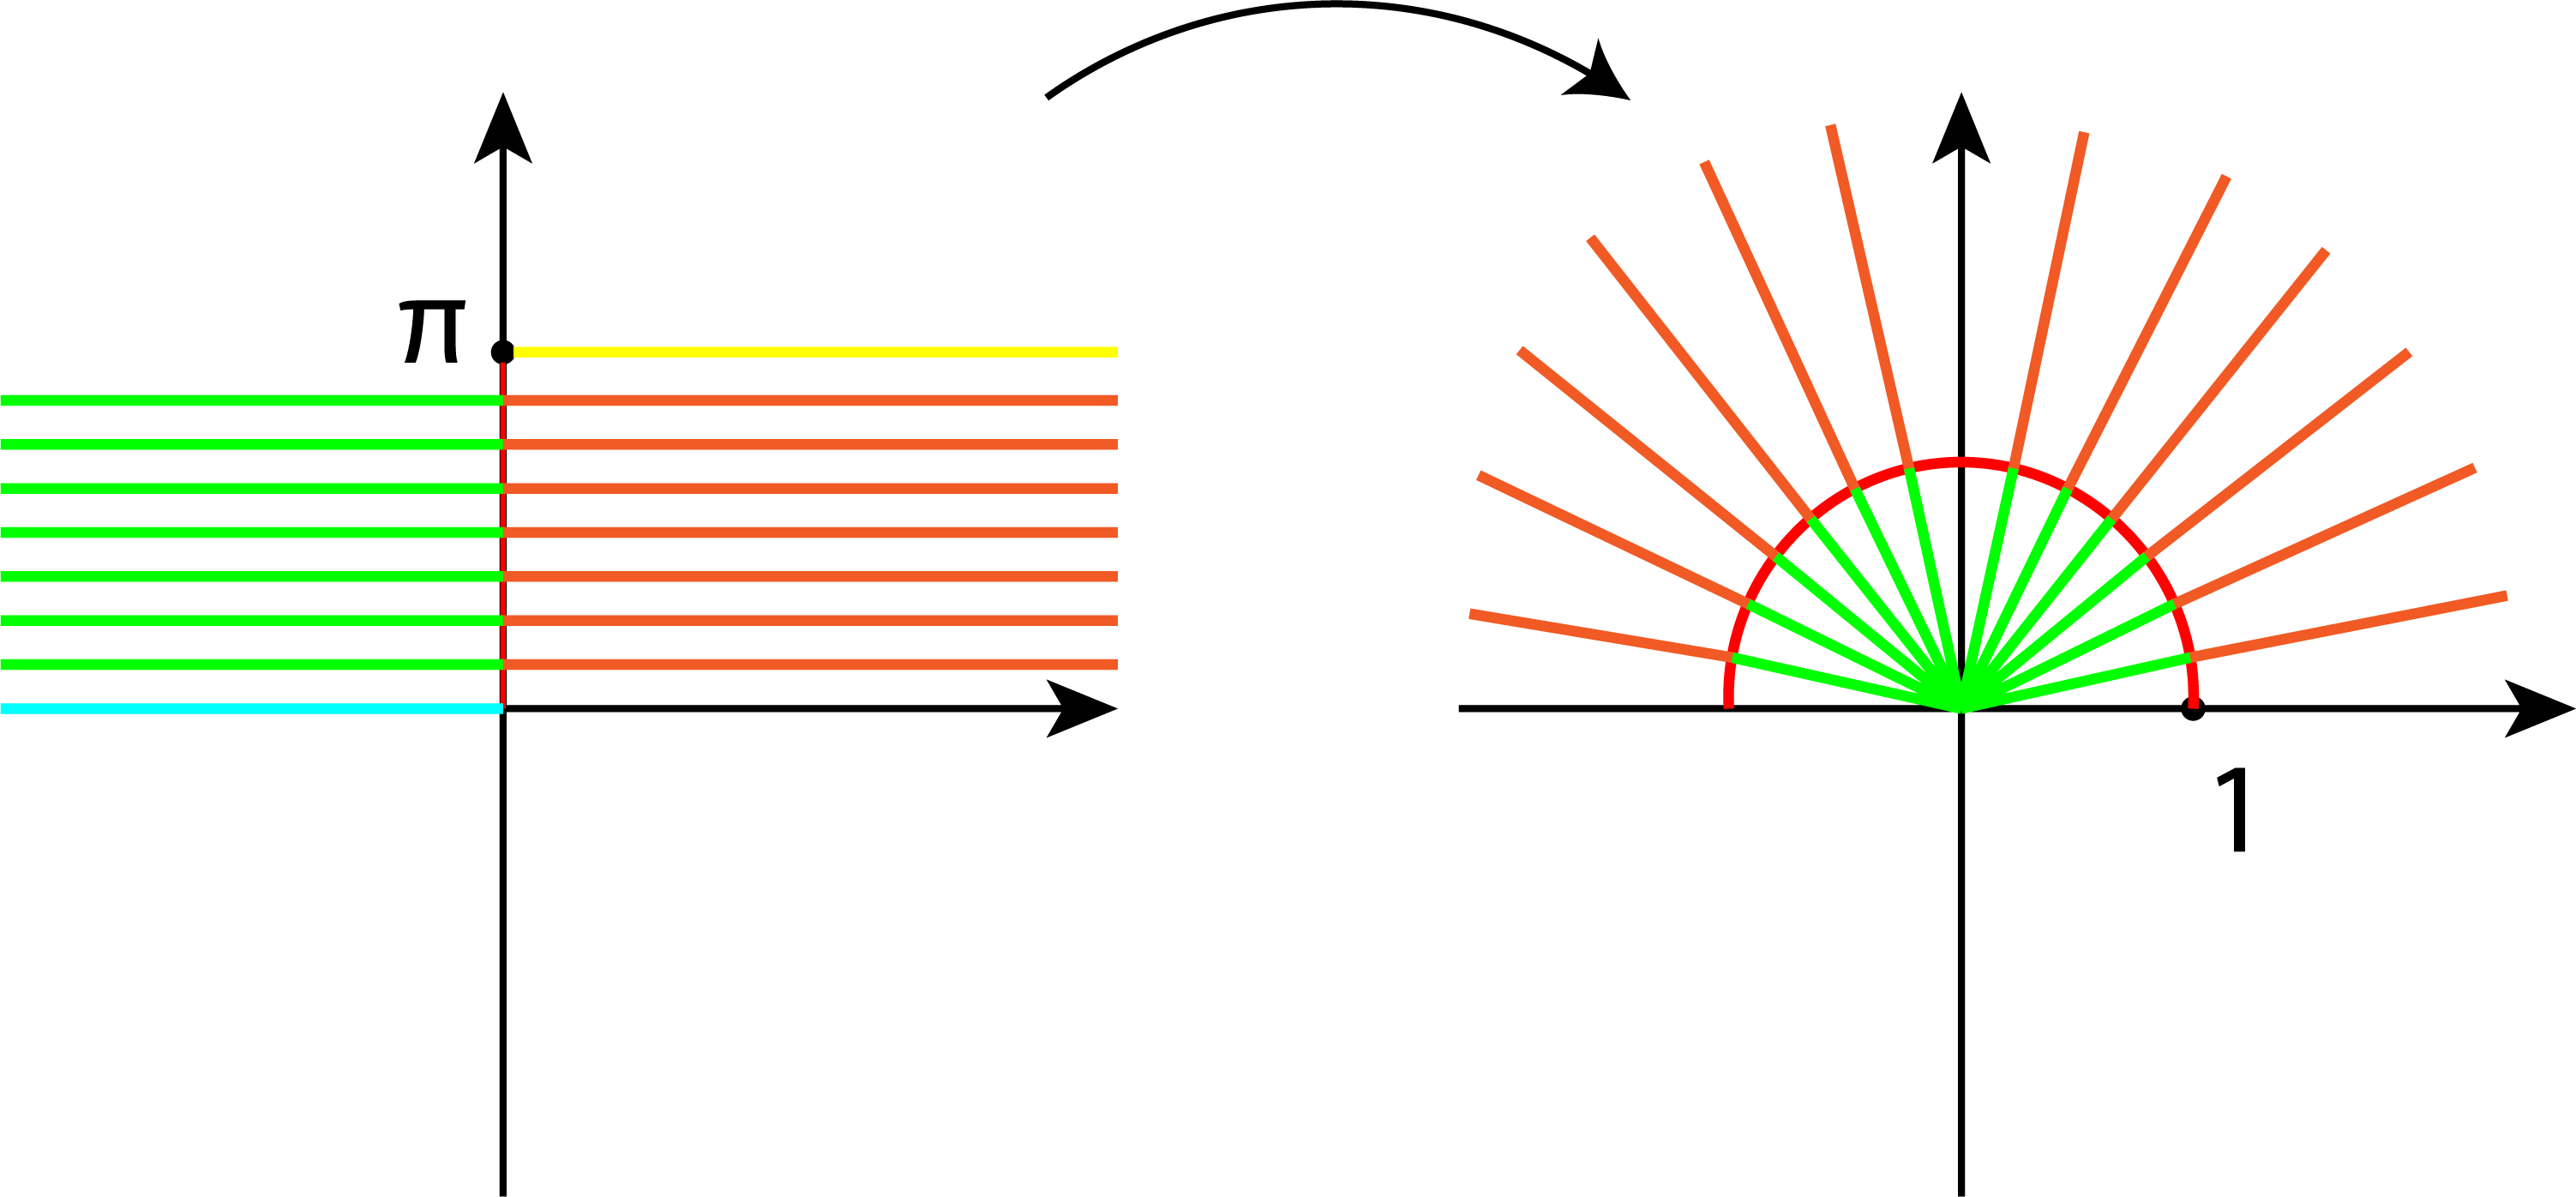
\includegraphics[width=8cm]{8_12}
		\end{figure}
		\[\begin{cases}
			y = 0\\
			0 \leq x < \infty
		\end{cases} \os{e^z}{\to } e^x (\cos 0 + i \sin 0) = e^x \geq 1\]
		\[\begin{pmatrix}
			x = 0\\
			0 \leq y \leq \pi
		\end{pmatrix} \os{e^z}{\to } e^0 (\cos y + i\sin y)\]
		\[\begin{cases}
				y = \pi\\
				0 \leq x < +\infty
			\end{cases} \os{e^z}{\to} e^x (\underbracket{\cos \pi + i \sin \pi}_{-1}) = -e^x \leq -1\]
		hint: "для понимания можно представлять это как веер"
		\[e^z = e^x (\cos y + i \sin y) = e^x (\cos (y + 2 \pi k) + i \sin(y + 2 \pi k)) =\]
		\[ = e^{x + i(y + 2\pi k)} = e^{z + i \cdot 2 \pi k}  \]
		\[\text{Период } e^z \q T = e\pi k i\]
	\end{Example}

	\begin{Definition}["выводится"{} из ф. Эйлера]
		\[\sin z = \dfrac{e^{iz} - e^{-iz}}{2i}\]
		\[\sin z = -i \sh(iz)\]
		Период $f(z) = \sin z \q T = 2\pi k,\q k \in \Z$\\
		$g(z) = \sh z$ - период $2 \pi i$
		\[\cos z = \dfrac{e^{iz} + e^{-iz}}{2} = \ch(iz)\]
		\[\ch z = \dfrac{e^z + e^{-z}}{2}\]
	\end{Definition}

	\begin{Definition}
		\[\text{Ж}(z) = \frac{1}{2} \Br{z + \frac{1}{z}} \text{ --- \ul{функция Жуковского}}\]
		\[T = \{z : \abs{z} = 1\}\]
		\begin{figure}[H]
			\centering
			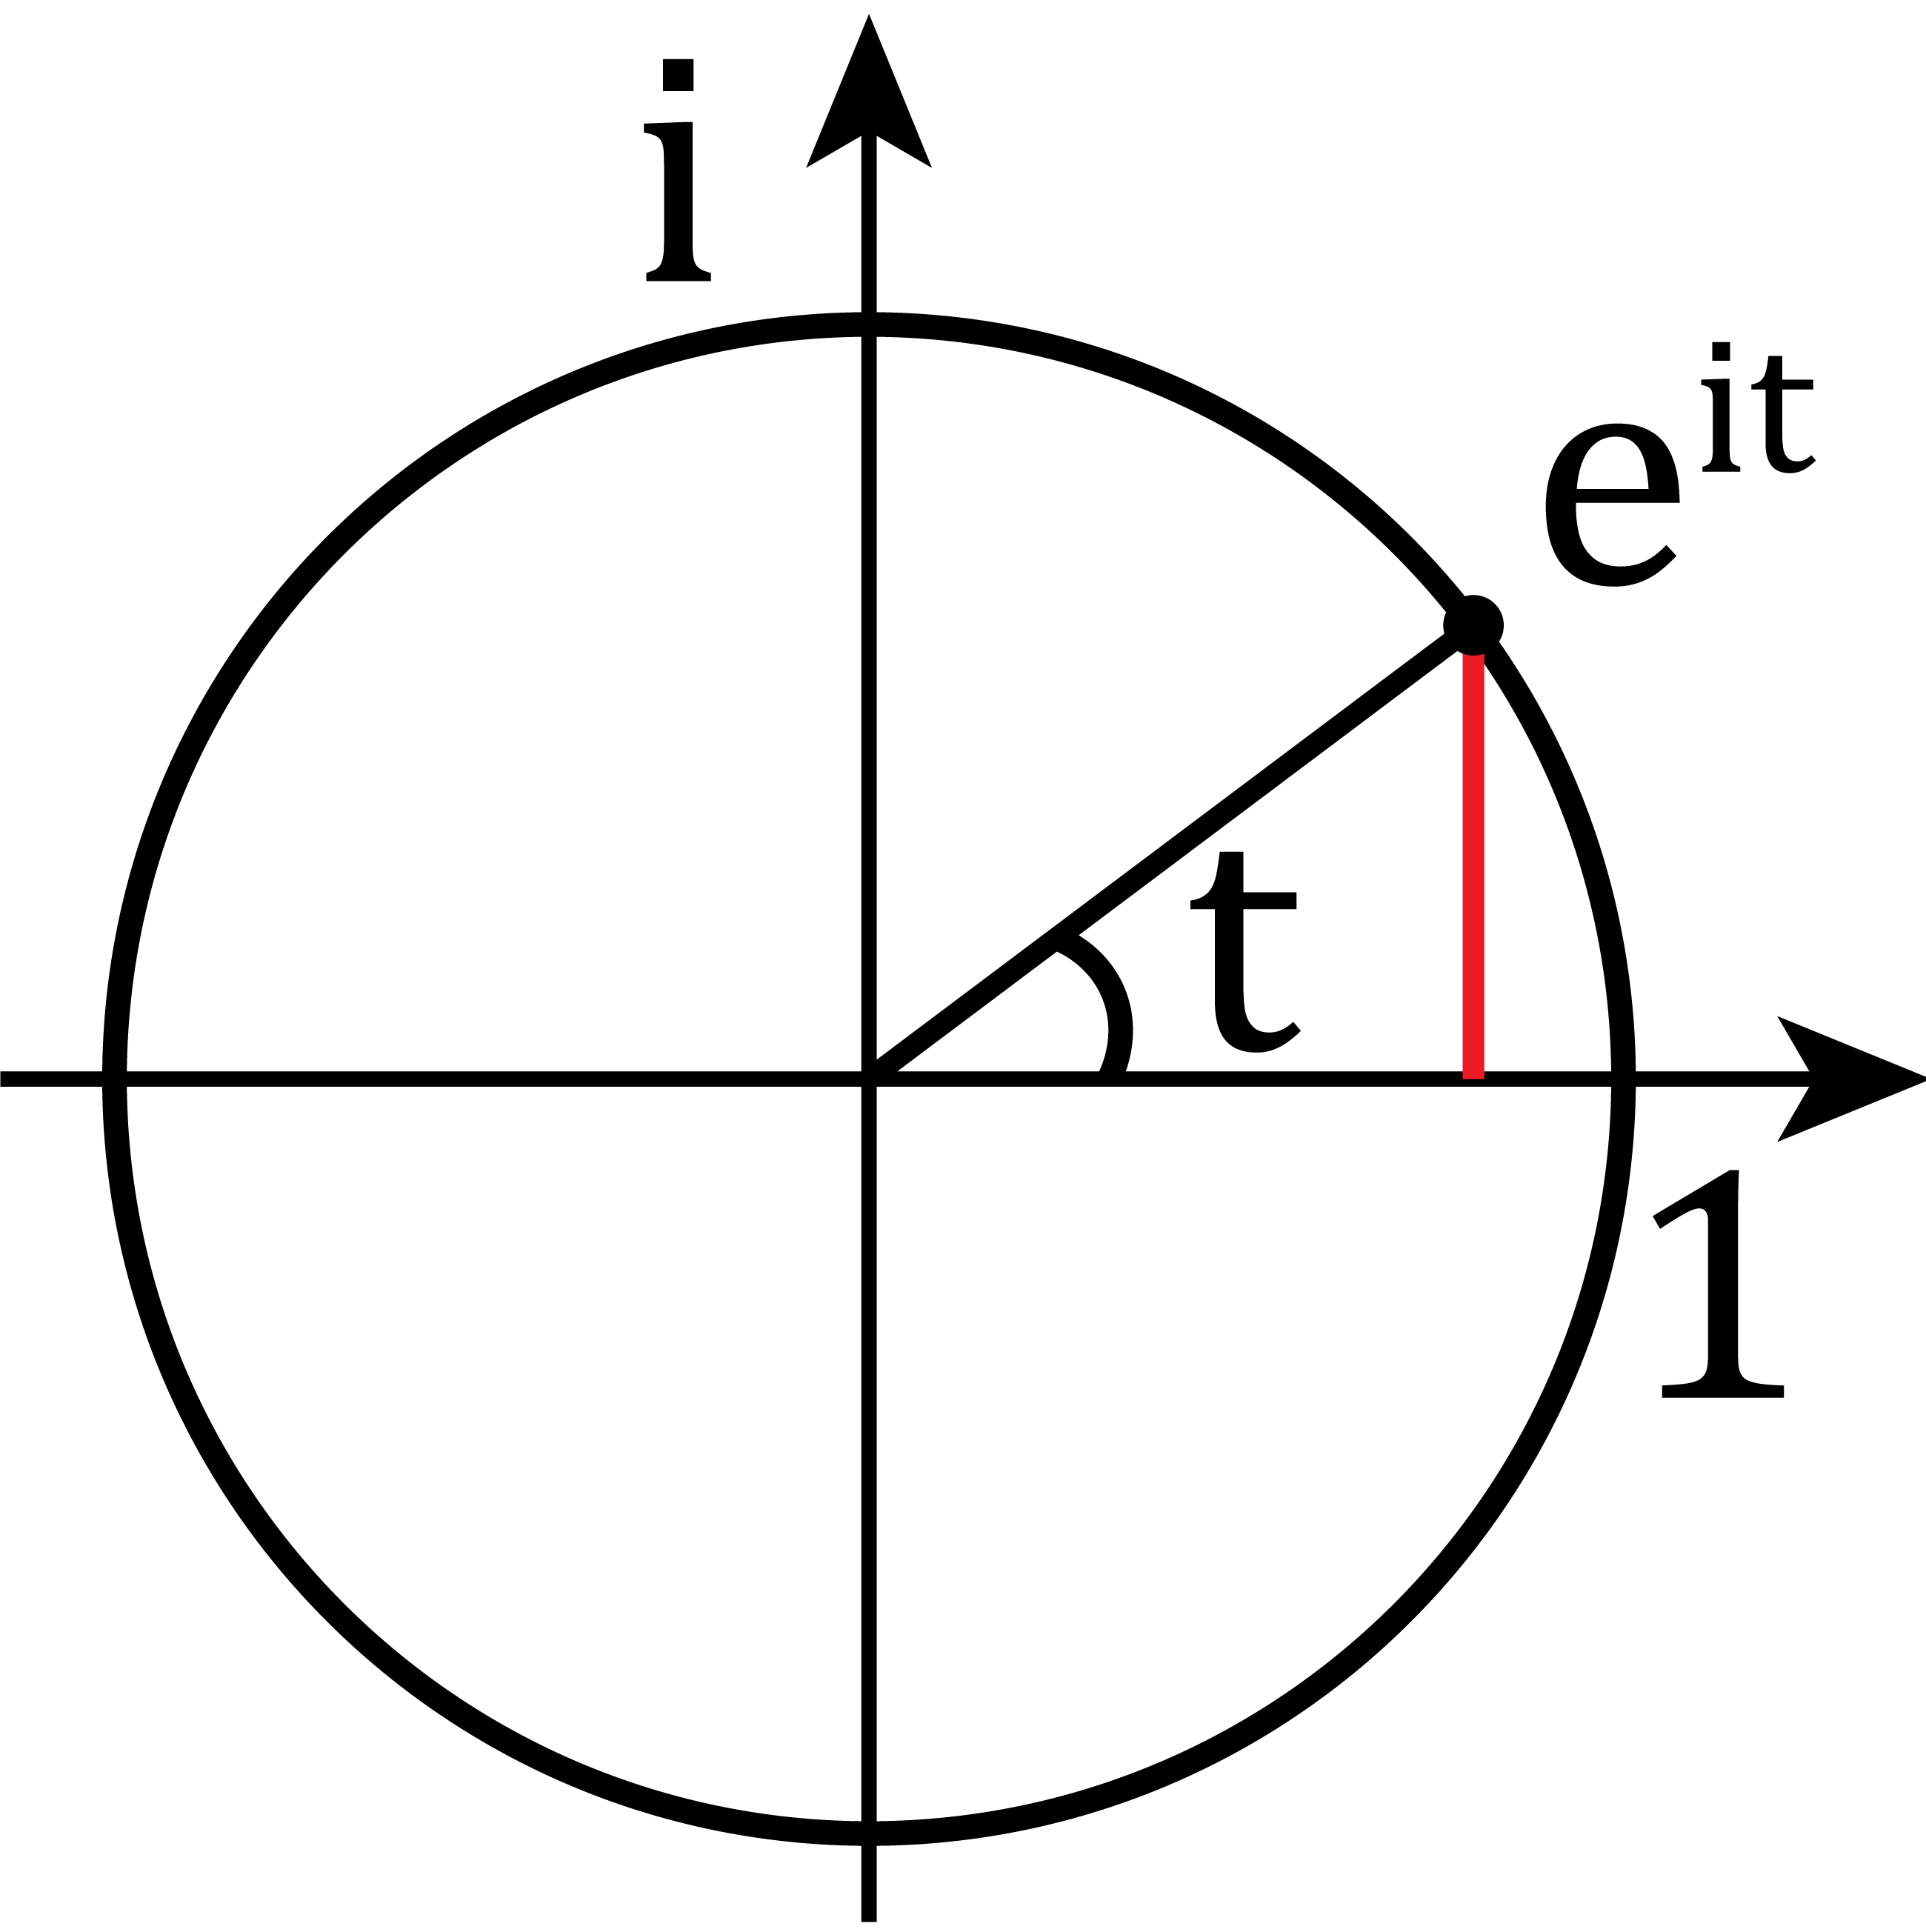
\includegraphics[width=3.5cm]{9_1}
		\end{figure}
		\[z = e^{it} = \cos t + i \sin t \]
		\[- \pi \leq t \leq \pi\]
		\[\text{Ж}(e^{it}) = \frac{1}{2} (e^{it} + e^{-it} ) = \cos t = \text{Ж}(e^{-it})\]
		\[\text{Ж}(T) = [-1, 1] \text{ не вз.-одн.} \] %?what не вз-одн?
		Прообраз $\forall a \in (-1, 1) $ сост. из двух т.
		\[rT = \{r e^{it}, -\pi \leq t \leq \pi\}\]
		\[0 < r < 1\]
		\[\text{Ж}(r e^{it}) = \frac{1}{2} \Br{r e^{it} + \frac{1}{r} e^{-it}} =
			\frac{1}{2} \Br{r + \frac{1}{r}} \cos t + i \frac{1}{2} \Br{r - \frac{1}{r}} \sin t\]
		\begin{figure}[H]
			\centering
			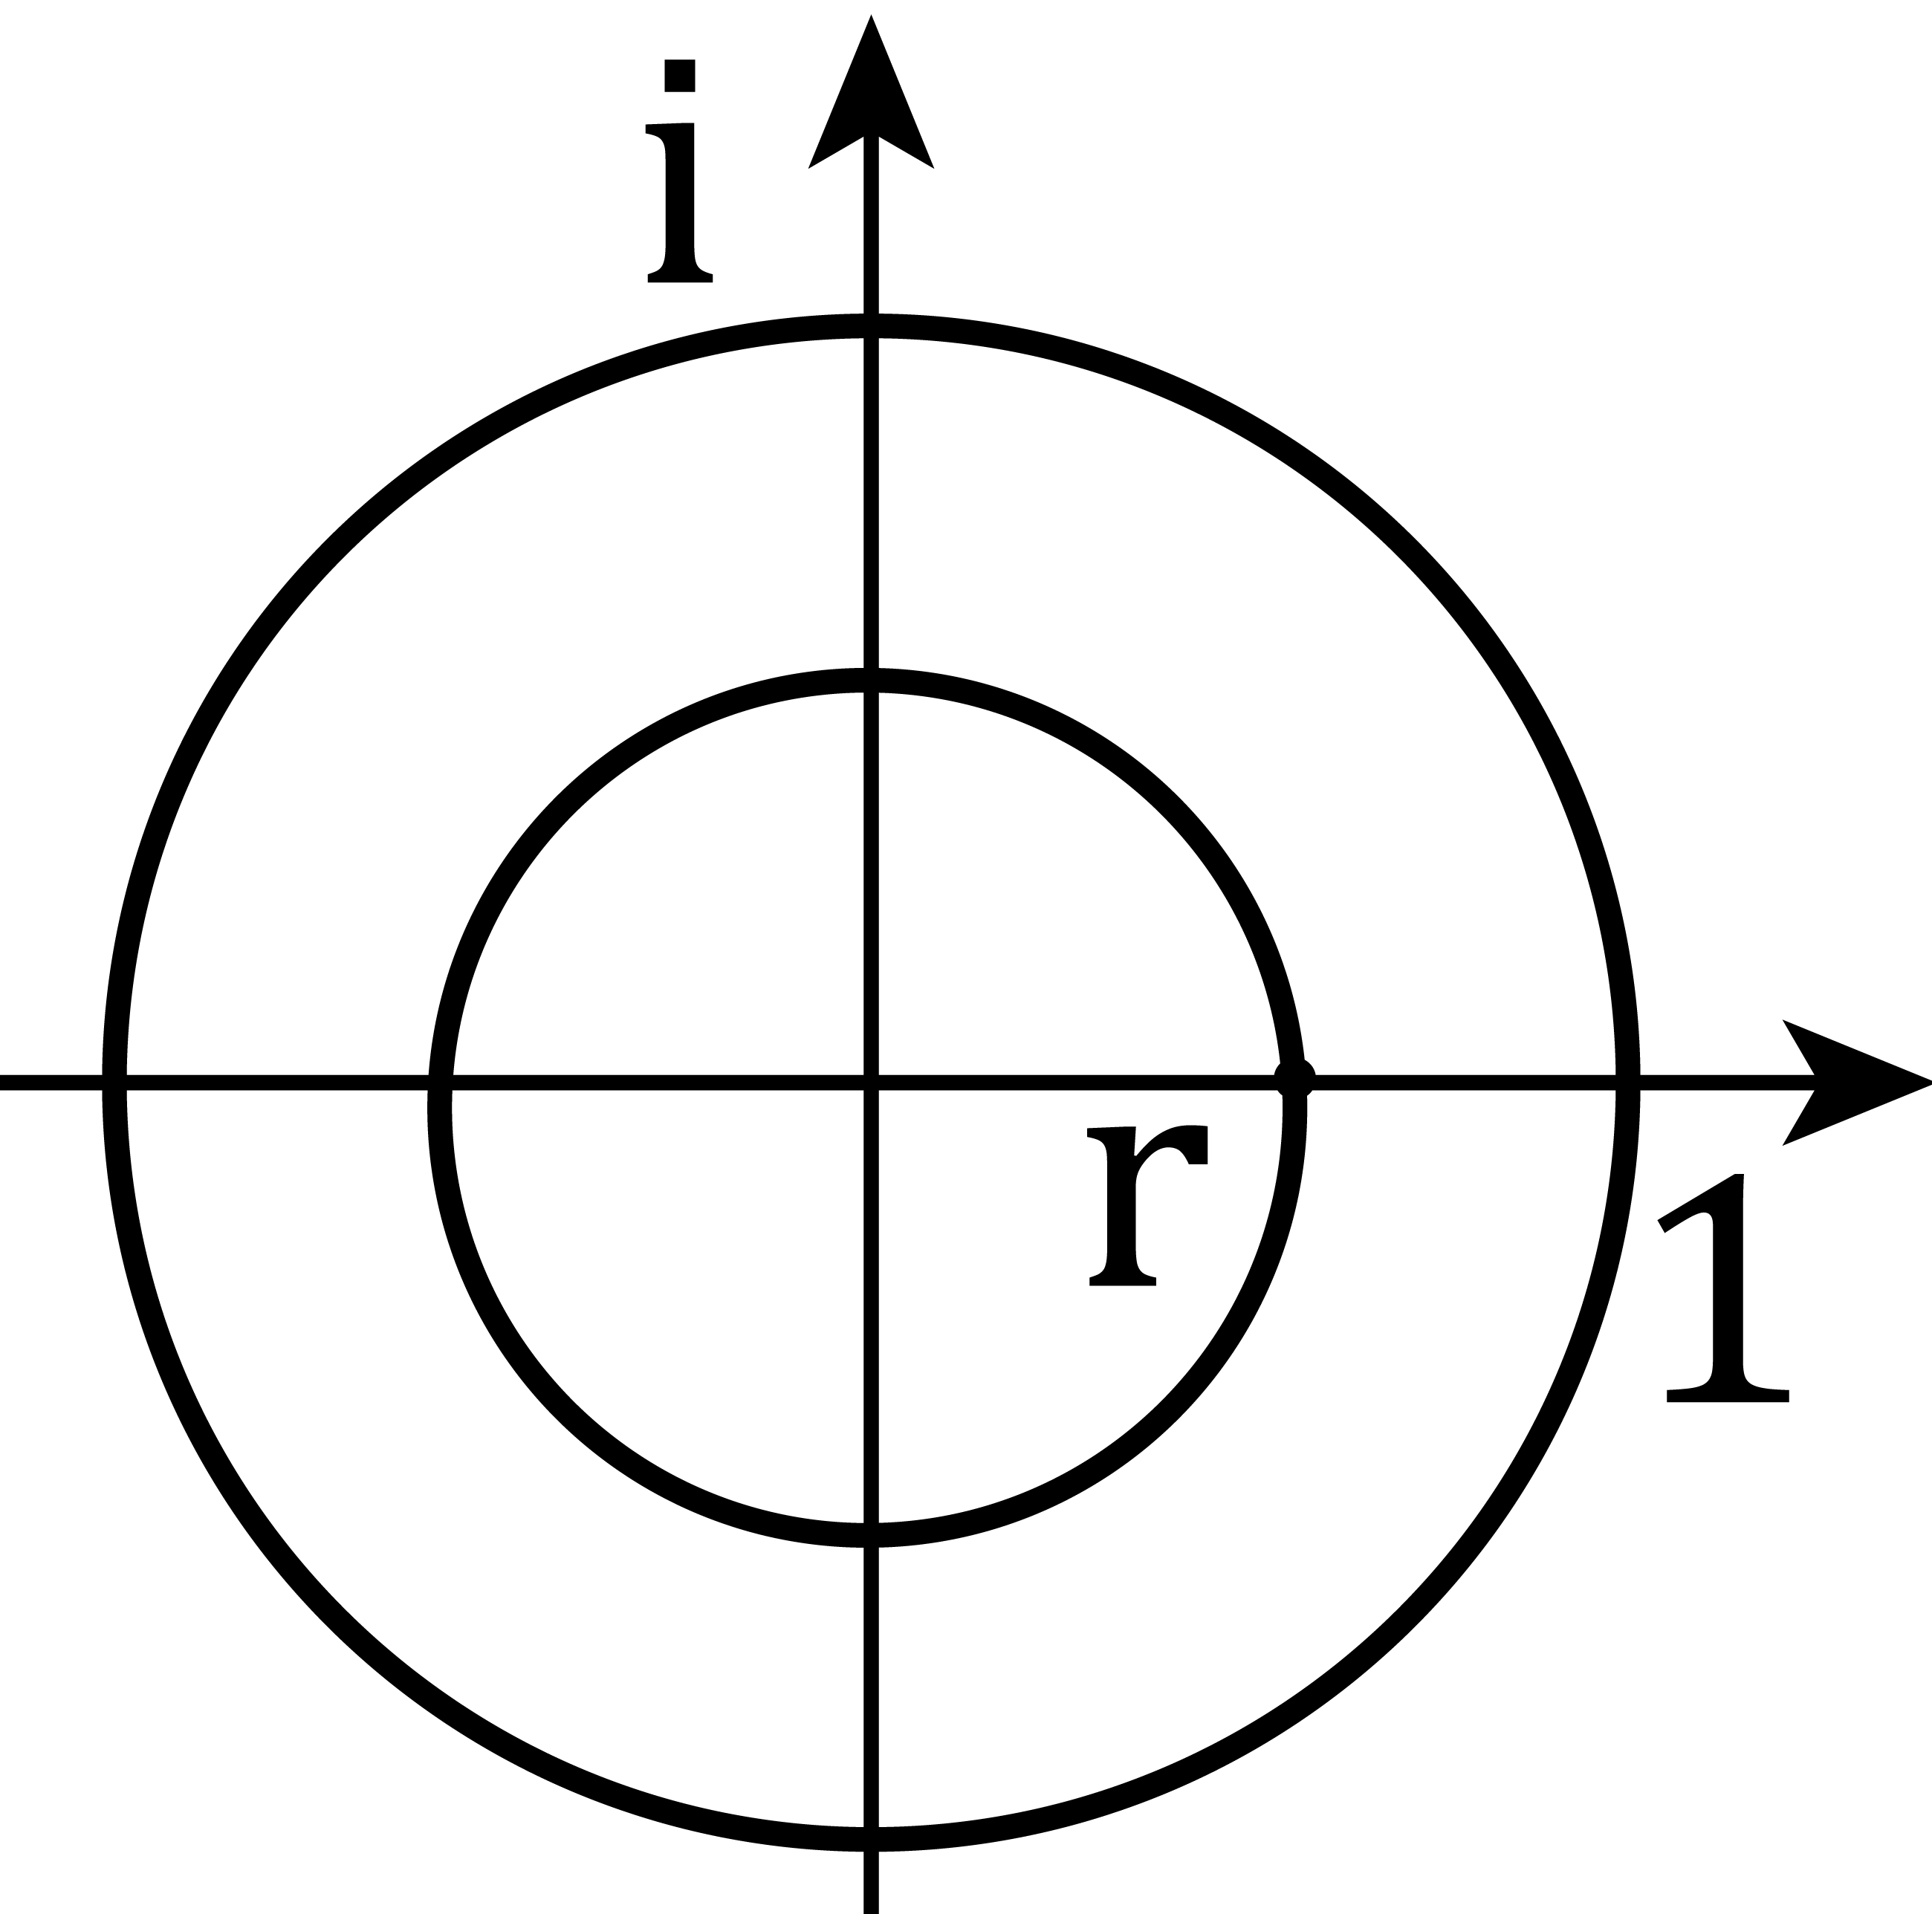
\includegraphics[width=3.5cm]{9_2}
		\end{figure}
		\[\begin{cases}
				\real \text{Ж} (r e^{it} ) = \frac{1}{2} (r + \frac{1}{r}) \cos t \\
				\im \text{Ж} (r e^{it} ) = \frac{1}{2}(r - \frac{1}{r}) \sin t
			\end{cases} \text{ --- пар. ур. эллипса с полуосями}\]
		\[a = \frac{1}{2} \Br{r + \frac{1}{r}} \geq 1\]
		\[b = \frac{1}{2} \Br{\frac{1}{r} - r}\]
		\[-\pi \leq t \leq \pi\]
		\begin{figure}[!h]
			\centering
			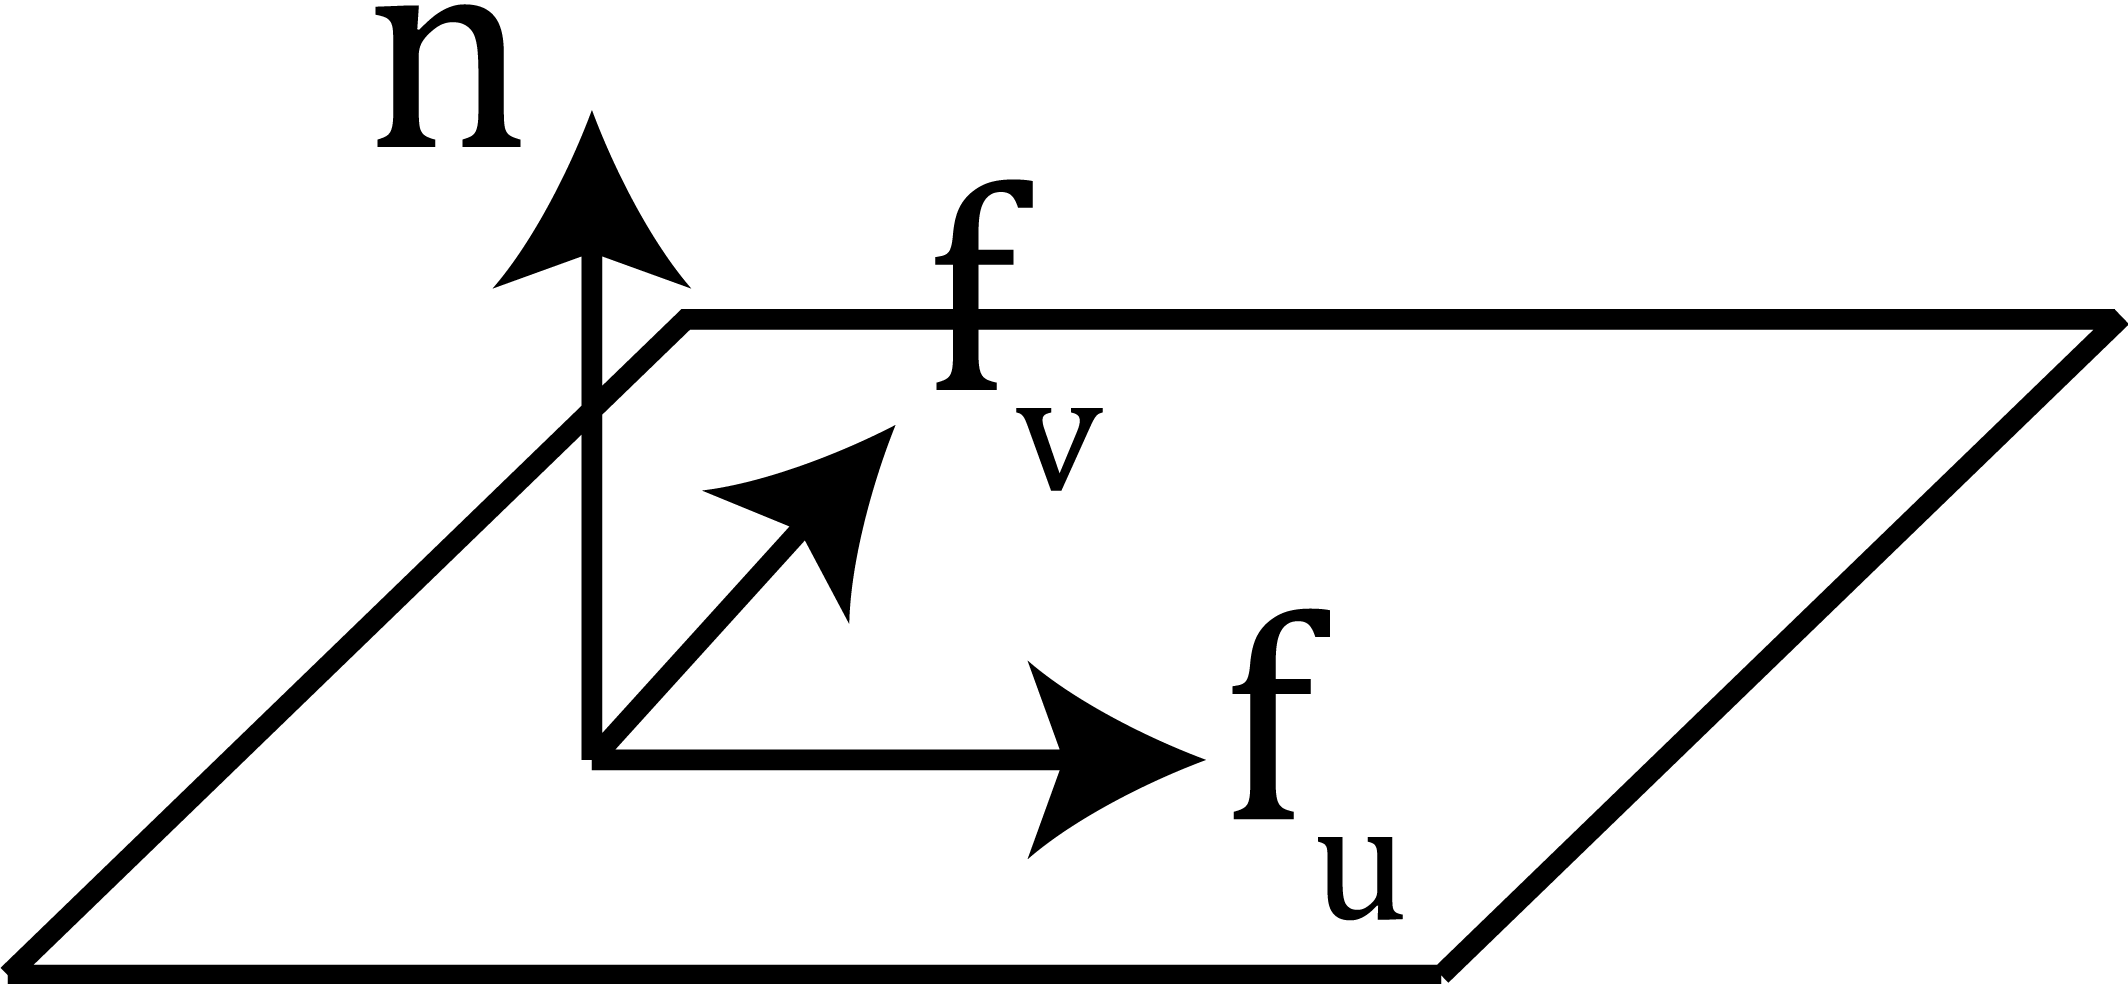
\includegraphics[width=7cm]{9_3}
		\end{figure}
		\[R > 1 \qq \text{Ж} (R e^{it} ) = \frac{1}{2} \Br{\ub{\geq 1}{R + \frac{1}{R}}}\cos t + i \frac{1}{2}
			\Br{\ub{\geq 0}{R - \frac{1}{R}}} \sin t\]
		\[\cos z = \frac{e^{iz} + e^{-iz}}{z} = \text{Ж}(e^{iz} )\]
		\begin{figure}[H]
			\centering
			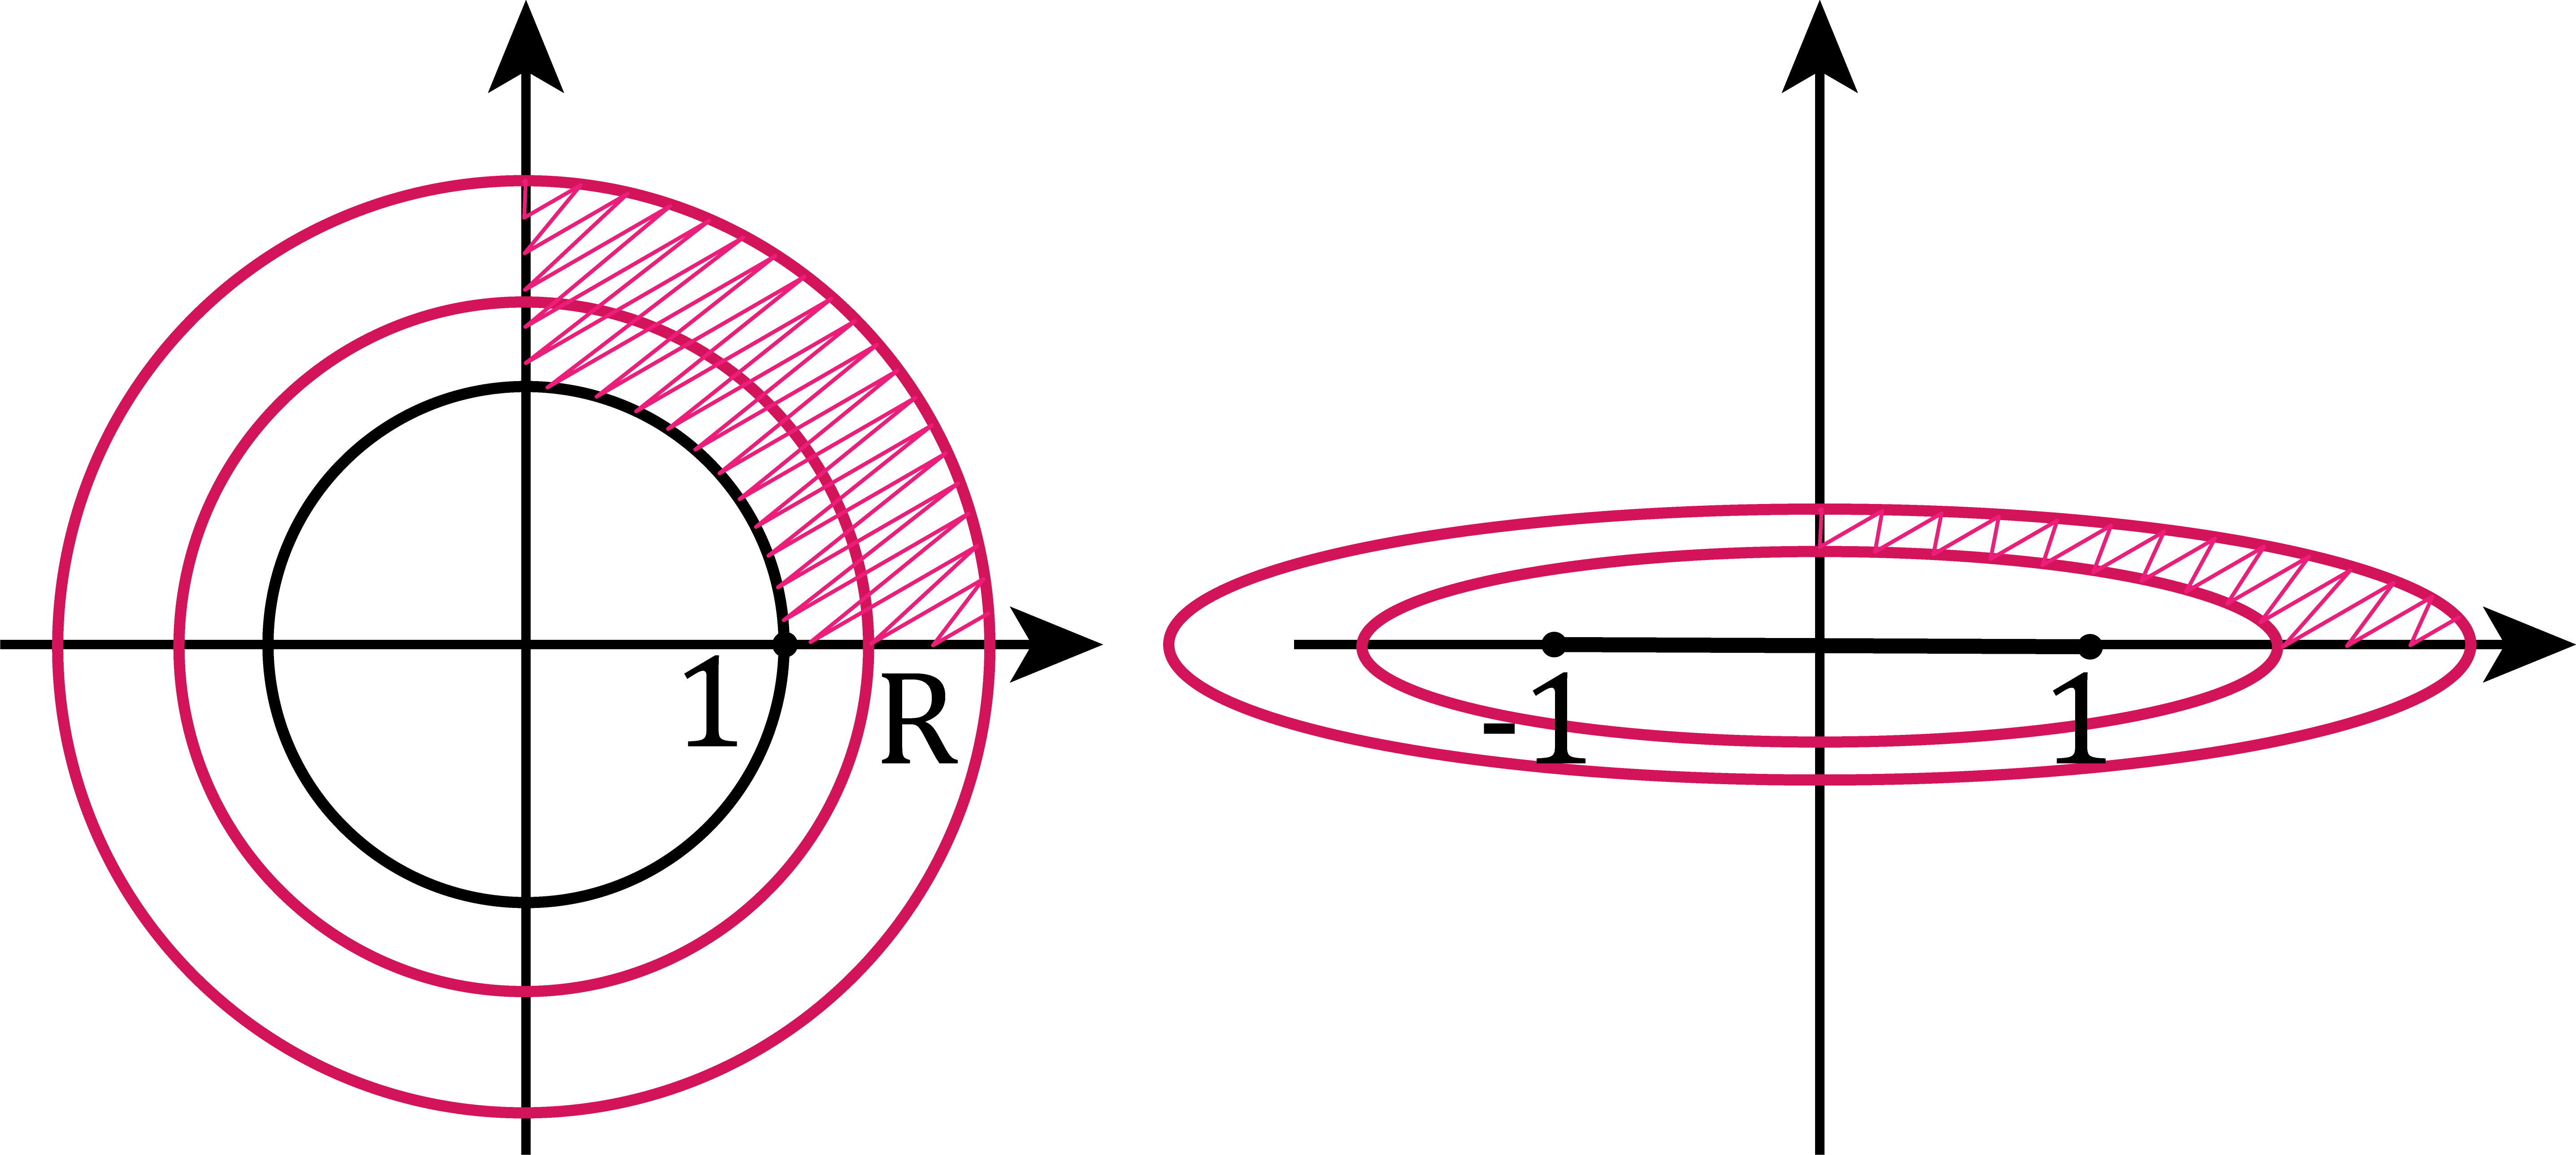
\includegraphics[width=7cm]{9_4}
		\end{figure}
	\end{Definition}

	\begin{Definition} [аргумент комплексного числа]
		\[z = x + iy; \q \abs{z} = \sqrt{x^2 + y^2}\]
		\begin{figure}[H]
			\centering
			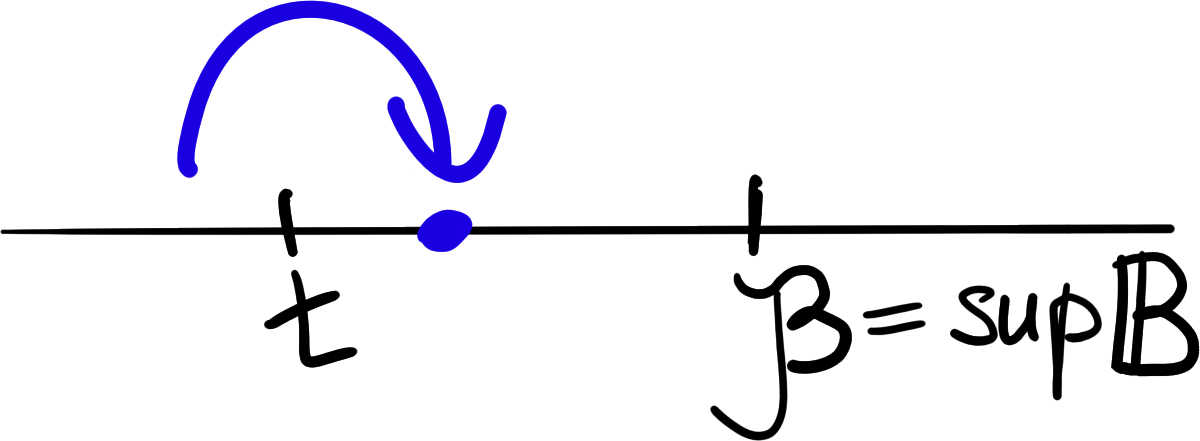
\includegraphics[width=3cm]{9_5}
		\end{figure}
		\[z \to \abs{z}; \text{ угол } \varphi \qq z = \abs{z} (\cos \varphi + i \sin \varphi)\]
		Подходят все углы $\varphi + 2 \pi k, \q k \in \Z$
		\[\Arg z = \{\varphi + 2\pi k, \q k \in \Z\} \text{ --- \ul{полное значение аргумента}}\]
		Отображение $\Arg : \CC \to $\\
		$\forall z \in \CC $ сопоставляет множество
	\end{Definition}

	\begin{Definition} [непрерывная ветвь аргумнта]
		\[\text{Ф-я } \alpha : \Omega \to \R \qq \Omega \subset \CC\]
		Называется \ul{непрерывной ветвью аргумента} $z$, если:
		\[\alpha \in C(\Omega) \text{ и } \forall z \in \Omega \q \alpha(z) \in \text{ Arg} z\]
	\end{Definition}

	\begin{Example}
		\[\Omega = \{\abs{z} < 1\} \text{ здесь нельзя определить однозн. ветвь аргумента}\]
		\begin{figure}[H]
			\centering
			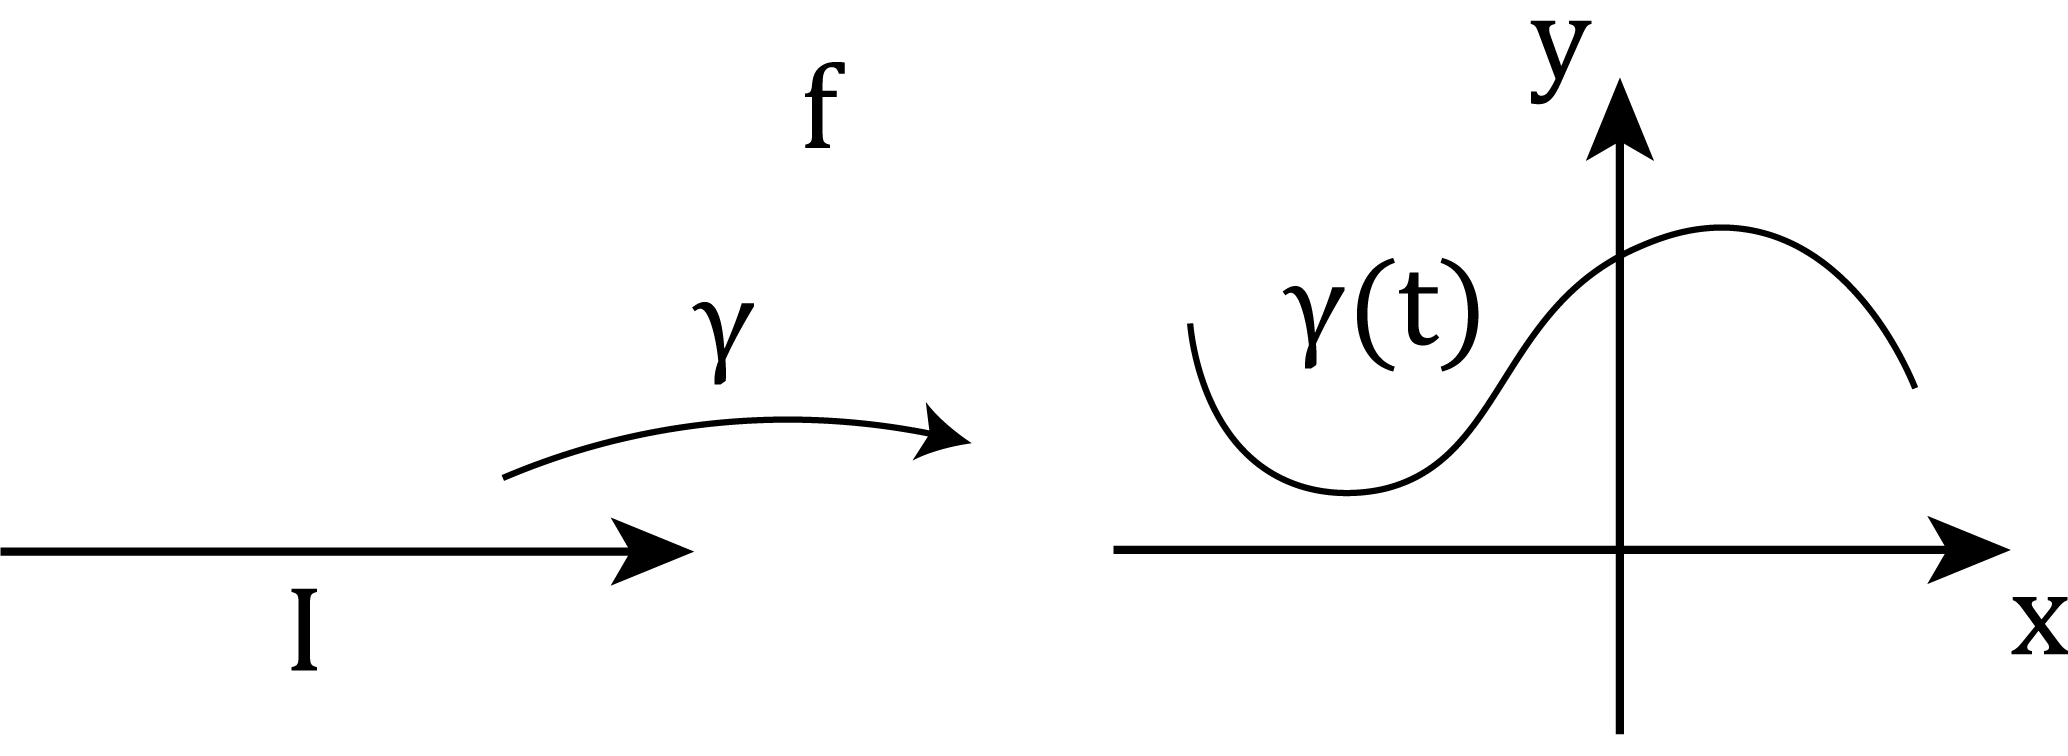
\includegraphics[width=3.5cm]{9_6}
		\end{figure}
		\[\Omega = \CC \setminus \{z = x;\q x \in (- \infty, 0]\}\]
		Главное значение аргумента
		\[\begin{cases}
				\arg (z) \in \Arg(z) \\
				\arg (z) \in (-\pi, \pi)
			\end{cases}\]
		\[z = x < 0 \qq \arg(z) = \pi\]
		\[\Arg z = \{\arg z + 2 \pi k, k \in \Z\}\]
		\[\Arg z = \arg z + 2 \pi k\]
	\end{Example}

	\begin{Example} [некоторые многозначные функции]
		\[w^n = z, \q n \in \N\]
		Уравнение имеет $n$ решений
		\[w = \abs{w} \cdot e^{i \Arg w}  \q z = \abs{z} \cdot e ^{i \Arg z} \]
		\[\begin{cases}
				\abs{w}^n = \abs{z} \\
				n \Arg w = \Arg z
			\end{cases}\]
		\[\abs{w} = \us{\R}{\sqrt[n]{\abs{z}}} \qq \us{\R}{\sqrt[n]{x}} = x^{\frac{1}{n}}  \q x \in \R\]
		\[n \Arg w = \arg z + 2 \pi k, \q k \in \Z\]
		\[\Arg w = \left\{\frac{\arg z}{n} + \frac{2 \pi k }{n}, \q k \in \Z\right\}\]
		\[w = \us{\CC}{\sqrt[n]{z}} = \us{\R}{\sqrt[n]{\abs{z}}} \cdot e^{i (\frac{\arg z}{n} +
					\frac{2 \pi k }{n})} \]
		\[\forall z \in \CC \setminus \{0\}\]
		\[\sqrt[n]{z} \text{ принимает } n \text{ разл. знач.}\]
	\end{Example}

	\begin{Definition} [комплексный логарифм]
		\[e^w = z\]
		\[w = u + iv\]
		\[e^{u + iv} = e^u \cdot e^{iv} = \abs{z} \cdot e^{i \text{Arg z}} \]
		\[\begin{cases}
				e^u = \abs{z} \\
				v = \Arg z
			\end{cases} \qq \begin{cases}
				u = \us{\R}{\ln} \abs{z} \\
				v = \arg z + 2 \pi k
			\end{cases}\]
		\[w = \us{\R}{\ln} \abs{z} + i (\arg z + 2\pi k) = \us{\R}{\ln } \abs{z} + i \Arg z\]
		\[\ln z = \us{\R}{\ln}\abs{z} + i \arg z\]
		Если $x > 0$, то arg $x$ = 0
		\[\ln x = \us{\R}{\ln} x + i0\]
		\[\Ln z = \ln \abs{z} + i \Arg z \text{ --- \ul{комплексный логарифм}}\]
		\[\Ln z = \ln z + 2 \pi k i\]

		\[a, b \in \CC \q a \neq 0\]
		\[a^b = e ^ {(\text{Ln a})b}\]
		\[i^i = e^{(\Ln i)i} \]
		\[\Ln i = \ln \abs{i} + i \Arg i = 0 + i \Br{\frac{\pi}{2} + 2 \pi k}\]
	\end{Definition}

	\begin{Definition} [обратные тригонометрические функции]
		\[\cos w = z\]
		\[e^{iw} + e^{-iw} = 2z\]
		\[e^{iw} = t \qq t^2 - 2t \cdot z + 1 = 0\]
		\[t = z + \sqrt{z^2 - 1} = e^{iw} \]
		\[iw = \Ln \Br{z + \sqrt{z^2 - 1}}\]
		\[\arccos z = -i \cdot \Ln \Br{z + \sqrt{z^2 - 1}}  \os{*}{=}\]
		\[z + \sqrt{z^2 - 1} = \frac{1}{z - \sqrt{z^2  - 1}}\]
		\[\os{*}{=} i \Ln \Br{z - \sqrt{z^2 - 1}}\]
	\end{Definition}

	\begin{Example}
		\[\text{Решим уравнение } \sin z = i\]
		\[e^{iz} - e^{-iz} = 2i^2 = -2  \]
		\[e^{iz}  = t\]
		\[t^2 + 2t - 1 = 0\]
		\[t = -1 + \us{\CC}{\sqrt{1 + 1}} = \pm \us{\R}{\sqrt{2}} - 1 \qq \sqrt{2} - 1 = \frac{1}{\sqrt{2} + 1}\]
		\[iz = \Ln (\pm \sqrt{2} - 1)\]
		\[\bigg[\begin{align}
				 & iz = \ln(\sqrt{2} - 1) + i (2 \pi k)          \\
				 & iz = \ln(-\sqrt{2} - 1) + i (\pi + 2 \pi k) =
			\end{align}\]
		\[ = \ln\Br{- \frac{1}{\sqrt{2} - 1}} + i (\pi + 2\pi k) = -\ln(\sqrt{2} - 1) + i 2 \pi k\]
	\end{Example}

	\newpage
	\subsection{Комплексное дифференцирование. Условия Коши-Римана}

	\begin{Definition}
		\[\Omega \subset \CC \qq \Omega \text{ --- \ul{область}, если:}\]
		\begin{enumerate}
			\item $\Omega$ --- откр.
			\item $\forall a, b \in \Omega \q$ можно соед. ломаной ($\Omega$ --- связно)
		\end{enumerate}
	\end{Definition}

	\begin{Definition}
		\[f : \Omega \to \CC \qq z_0 \in \CC\]
		\[f \text{ --- \ul{диф-ма ($\CC$ --- диф-ма)} в т. $z_0$, если:}\]
		\[\exists A \in \CC : \q f(z) = f(z_0) + A(z - z_0) + o(\abs{z - z_0}) \qq z \to z_0\]
		\[A = \us{\text{произв. } f}{f'(z_0)} = \lim_{z \to z_0} \frac{f(z) - f(z_0)}{z - z_0} =
			\lim_{\Delta z \to 0} \frac{f(z_0 + \Delta z) - f(z_0)}{\Delta z} \]
		\[z - z_0 = \Delta z\]
		Предел не зависит от того, как $\Delta z \to 0$
	\end{Definition}

	\begin{Example} [1]
		\[f(z) = \overline{z} \qq z_0 = 0\]
		\[f'(0) =? \lim_{\Delta z \to 0} \frac{\overline{\Delta z} - 0}{\Delta z} =
			\lim_{\Delta \to 0} \frac{\Delta x - i \Delta y}{\Delta x + i \Delta y} \]
		Если $\Delta z = \Delta x \to 0$, то $\displaystyle \lim_{\Delta z \to 0} \frac{\overline{\Delta z}}
			{\Delta z} = 1 $ \\
		Если $\Delta z = i\Delta y \to 0$, то $\displaystyle \lim_{\Delta z \to 0} \frac{\overline{\Delta z}}
			{\Delta z} = -1 $
	\end{Example}

	\begin{Example} [2]
		\[f(z) = z^n, \q n \in \N\]
		\[f'(z_0) = \lim_{\Delta z \to 0} \frac{(z_0 + \Delta z)^n - z_0^n}{\Delta z} = \]
		\[ = \lim_{\Delta z \to 0} \frac{z_0^n + n \Delta z z_0^{n - 1} + C^2_n \Delta z^2 z_0^{n - 2} + ...+
			\Delta z^n - z_0^n}{\Delta z} = n \cdot z_0^{n - 1}  \]
	\end{Example}

	\begin{theorem} [основные правила диф-я]
		\begin{enumerate}
			\item $(f + g) = f' + g'$
			\item $(\const \cdot f)' = \const \cdot f'$
			\item $(f \cdot g)' = f'g + fg'$
			\item $[f(g(z))]' = f'(g(z)) \cdot g'(z)$
		\end{enumerate}
	\end{theorem}

	\begin{utv}
		Если $f$ --- диф-ма в т. $z_0$, то она непр. в $z_0$
	\end{utv}

	\begin{Proof}
		\[f(z) - f(z_0) = f'(z_0) \cdot (z - z_0) + o(\abs{z - z_0}) \q z \to z_0\]
		\[\Ra f(z) \to f(z_0) \q z \to z_0\]
	\end{Proof}

	\begin{Definition}
		\[\us{\text{Область}}{\Omega \subset \CC} \qq z = x + iy \in \CC \leftrightarrow (x, y) \in \R\]
		\[f : \Omega \to \CC \qq f(z) = u(x, y) + iv(x, y)\]
		\[z \to (x, y) \to u(x, y) = \real f (x + iy)\]
		\[\q\q\q\q\q\q v(x, y) = \im f(x + iy)\] % костыль хы
		\[\begin{matrix}
			u : \Omega \to \R\\
			v : \Omega \to \R
		\end{matrix}\qq \begin{pmatrix}
				u \\
				v
			\end{pmatrix} : \Omega \to \R^2\]
	\end{Definition}

	\begin{Theorem} [условие Коши-Римана (Эйлера-Даламбера)]
		\[\us{\text{Область}}{\Omega \subset \CC},\q f : \Omega \to \CC \qq f(x + iy) = u(x, y) + iv(x, y)\]
		Следующие условия равносильны:
		\begin{enumerate}
			\item $f$ --- диф-ма $(\CC)$ в т. $z_0 \in \Omega$
			\item $u, v$ --- диф-мы в т. $(x_0, y_0)\q z_0 = x_0 + i y_0$
		\end{enumerate}
		\[\begin{cases}
				\dfrac{\partial u}{\partial x} (x_0, y_0) = \dfrac{\partial v}{\partial y}(x_0, y_0) \\
				\\
				\dfrac{\partial u}{\partial y} (x_0, y_0) = -\dfrac{\partial v}{\partial x}(x_0, y_0)
			\end{cases}\]
	\end{Theorem}

	\begin{proof}
		$(1 \Ra 2)$:
		\[\text{Предположим, что } f \text{ --- диф-ма в т. } z_0 \qq \Delta z = z - z_0\]
		\[f(z) = f(z_0) + f'(z_0) \cdot \Delta z + o(\abs{\Delta z}) \qq f(z) = u + iv\]
		\[f'(z_0) = A = a + ib \qq z = \Delta x + i\Delta y\]
		\[o(\abs{\Delta z}) = \us{\us{\Delta z \ra 0}{\ra} 0}{h(\Delta z)} \cdot \abs{\Delta z}
			= (\alpha(\Delta x, \Delta y) + i \beta (\Delta x, \Delta y)) \abs{\Delta z}\]
		\begin{multline*}
			u(x, y) + iv(x, y) = u(x_0, y_0) + iv(x_0, y_0) + (a + ib)(\Delta x + i\Delta y) + \\
			+ (\alpha(\Delta x, \Delta y) + i\beta(\Delta x, \Delta y)) \abs{\Delta z}
		\end{multline*}
		\[u(x, y) = u(x_0, y_0) + a \cdot \Delta x - b \Delta y + \alpha(\Delta x, \Delta y) \sqrt{\Delta x^2 +
				\Delta y^2}
		\]
		\[v(x, y) = v(x_0, y_0) + b \cdot \Delta x + a \Delta y + \beta(\Delta x, \Delta y) \sqrt{\Delta x^2 +
				\Delta y^2}
		\]
		\[\alpha, \beta \to 0 \qq \sqrt{\Delta x^2 + \Delta y^2} \to 0\]
		т.о $u, v $ - дифф-мы в т. $(x_0, y_0)$
		\[\frac{\partial u}{\partial x}(x_0, y_0) = a \q \frac{\partial u}{\partial y}(x_0, y_0) = -b\]
		\[\frac{\partial v}{\partial x}(x_0, y_0) = b \q \frac{\partial v}{\partial y}(x_0, y_0) = a\]
		\[\Ra \begin{cases}
				\dfrac{\partial u}{\partial x}(x_0, y_0) =  & \dfrac{\partial v}{\partial y}(x_0, y_0) \\
				\\
				\dfrac{\partial u}{\partial y}(x_0, y_0) = - & \dfrac{\partial v}{\partial x}(x_0, y_0)
			\end{cases}\]
		Условие К-Р, Э-Д\\ \ \\
		$(2 \Ra 1)$:
		\[\text{Пусть } u, v : \Omega \to \R \text{ диф-мы в т. } (x_0, y_0)\]
		\[\circlesign{+}\begin{cases}
			u(x, y) = u(x_0, y_0) + \dfrac{\partial u}{\partial x}(x_0, y_0)\Delta x + \dfrac{\partial u}{\partial y}(x_0, y_0)
				\Delta y + \us{\us{\Delta z \to 0}{\ra 0}}{\alpha(\Delta x, \Delta y)} \abs{\Delta z}\\
			\\
			v(x, y) = v(x_0, y_0) + \dfrac{\partial v}{\partial x}(x_0, y_0) \Delta x +
				\dfrac{\partial v}{\partial y}(x_0, y_0)\Delta y + \us{\us{\Delta z \to 0}{\ra 0}}{\beta (\Delta x, \Delta y)} \abs{\Delta z}\ \big| \cdot i
		\end{cases}\]
		\[\frac{\partial u}{\partial x}(x_0, y_0) = \frac{\partial v}{\partial y}(x_0, y_0) =: a \in \R\]
		\[\frac{\partial u}{\partial y}(x_0, y_0) = -\frac{\partial v}{\partial x}(x_0, y_0) =: -b \in \R\]
		\begin{multline*}
			\circlesign{=} f(z) = u(x, y) + iv(x, y) =\\
			= f(z_0) + a \Delta x - \us{=i^2 b}{b \Delta y} + ib \Delta x + ia \Delta y +
				\us{\os{(*)}{=} \E}{(\alpha + i \beta)}\abs{\Delta z}
		\end{multline*}
		\[\text{(*): т.к. $\alpha, \beta \ra 0$, то $\ra 0$ при $\Delta z \ra 0$}\]
		\[\Delta z \to 0\]
		\[f(z) = f(z_0) + \ub{= (a + ib) \Delta z}{(a + ib)\Delta x + i(a + ib)\Delta y} + \us{\ra 0}{\mathcal{E}}\abs{\Delta z}\]
	\end{proof}

	\begin{Remark}
		\[f'(z_0) = a + ib = u'_x(x_0, y_0) + iv'_x(x_0, y_0) = v'_y - i u'_y = u'_x - iu'_y = v'_y + iv'_x\]
	\end{Remark}

    \newpage
    \subsection{Теорема (условия, достаточные для постоянства аналитической функции)}

	\begin{Theorem}
		\[\us{\text{область}}{\Omega \subset \CC} \qq f : \Omega \to \CC \qq \]
		Предположим, что $f$ - диф-ма $\forall z \in \Omega$ и $f'(z) \in C(\Omega)$, тогда:
		\begin{enumerate}
			\item Если $f'(z) = 0 \q \forall z \in \Omega \RA f = const$
			\item Если $\real f(z) \equiv const \q \forall z \in \Omega \RA f(z) \equiv const \q \forall z \in \Omega$
			      \[(\im f = const \RA f = const)\]
			\item Если $\abs{f(z)} \equiv const \RA f(z) \equiv const$
			\item Если arg $f(z) \equiv const \RA f(z) \equiv const$
		\end{enumerate}
	\end{Theorem}

	\begin{Reminder} [лемма (т. о среднем)]
		\[f : U \to \R\]
		ч. пр. $f$ опр. $V_{x_0} \subset U  \q x \in V_{x_0}$
		\[\exists c^1, c^2 : \q f(x) - f(x_0) = \frac{\partial f}{\partial x}(c^1) \Delta x +
			\frac{\partial f}{\partial y}(c^2)\Delta y\]
	\end{Reminder}

	\begin{Proof}\
		%рисунок 6 с компактной кривой
        \begin{figure}[H]
            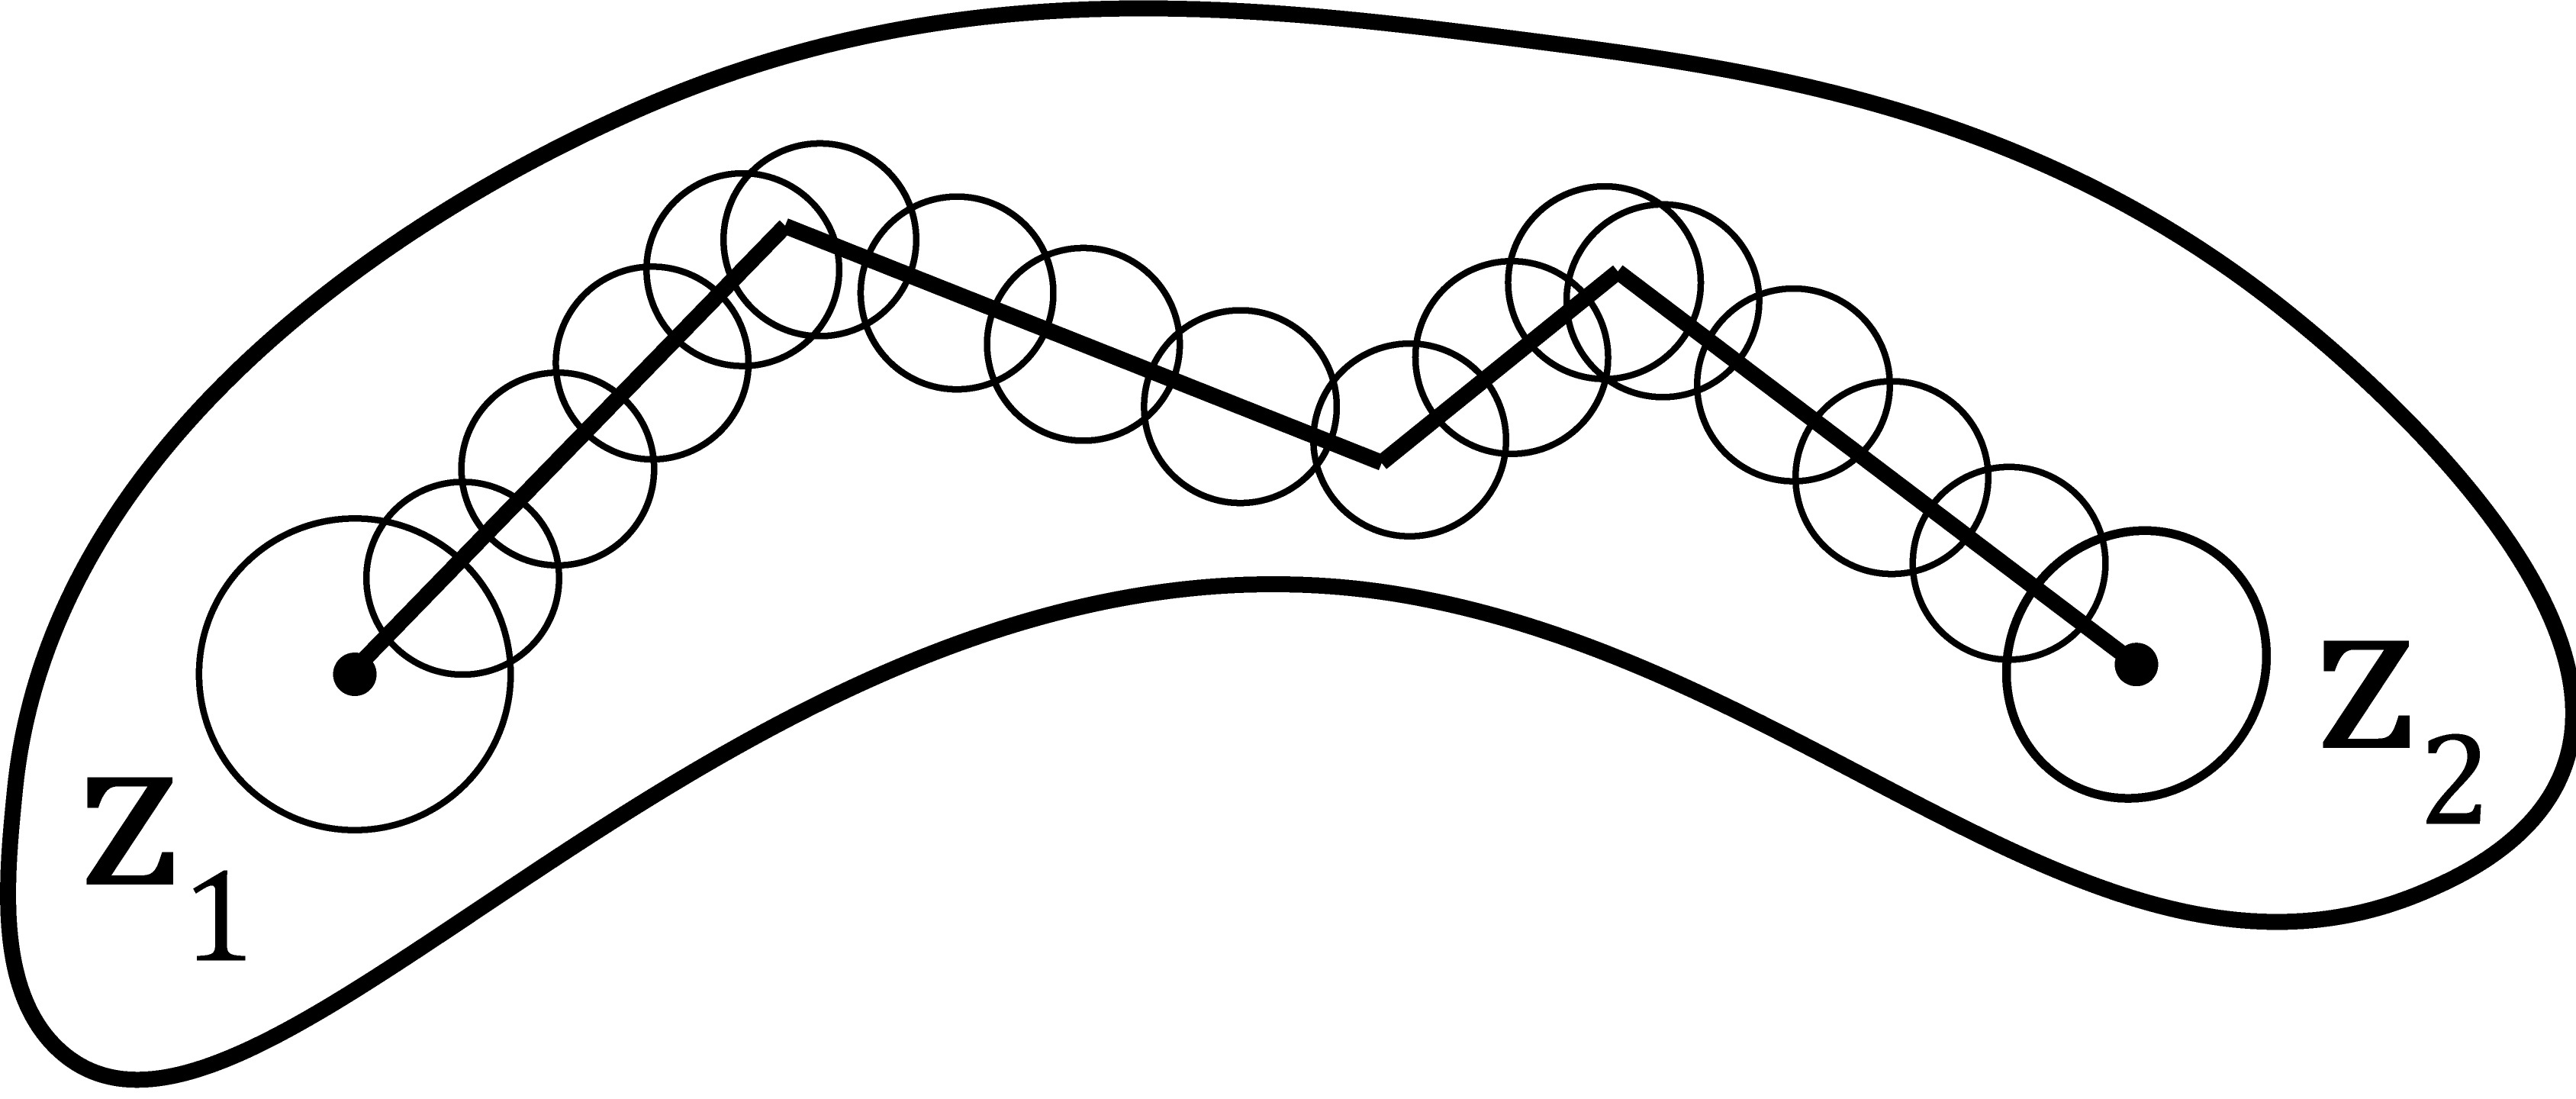
\includegraphics[width=5cm]{pics/9_8}
            \centering
        \end{figure}
		\begin{enumerate}
			\item $f'(z) = 0 = u'_x + i u'_y = v'_y + i v'_x$
				\[\begin{cases}
						u'_x \equiv 0 \\
						u'_y \equiv 0 \\
						v'_x \equiv 0 \\
						v'_y \equiv 0
					\end{cases} \qq \forall (x, y) \in \Omega\]
				По лемме $f(z_2) = f(z_1) \q \forall z_1, z_2 \in \Omega$
			\item $\real f = u(x, y) = const$
				\[\Ra\begin{cases}
						\dfrac{\partial u}{\partial x} (x, y) = 0 \\
						\\
						\dfrac{\partial u}{\partial y} (x, y) = 0
					\end{cases} \forall (x, y) \in \Omega \Ra (\text{+ К-Р}) \begin{cases}
						\dfrac{\partial v}{\partial y} = 0 \\
						\\
						-\dfrac{\partial v}{\partial x} = 0
					\end{cases}\]
				По лемме $v = \const $ в $\Omega$ $\Ra f(z) = \const$
			\item $\abs{f} = \const \Ra \abs{f}^2 = u^2 + v^2 = \const$
				\[\begin{cases}
						2 u \cdot u'_x + 2v v_x' = 0 \\
						2 u \cdot u'_y + 2v v'_y = 0
					\end{cases} \q \begin{cases}
						u \cdot u'x - v \cdot u'_y = 0 \\
						u \cdot u'y + v \cdot u'_x = 0
					\end{cases}\]
				Определитель системы л. ур
				\[\begin{vmatrix}
						u & -v \\
						v & u
					\end{vmatrix} = u^2 + v^2 \neq 0\]
				Если $u^2 + v^2 \neq 0 \Ra u'_x = 0, u'_y = 0 \Ra u \equiv \const \Ra v \equiv \const$
			\item $\arg f(z) \equiv \const \q \forall z \in \Omega$
				\[\text{Введем функцию } k = \frac{u}{v} \Ra k = \const\]
				\[\text{Дифф. } \forall z \in \Omega \q (1 + ik)f = (1 + ik)(u + iv) = u + iku + iv - u\]
				\[\real ((1 + ik)f) = 0 \Ra (1 + ik)f \equiv \const\]
		\end{enumerate}
	\end{Proof}
\end{document}
